\documentclass[10pt,letterpaper]{article}
\usepackage[top=0.85in,left=2.75in,footskip=0.75in]{geometry}
\usepackage[label font=Large,labelformat=simple]{subfig}
% amsmath and amssymb packages, useful for mathematical formulas and symbols
\usepackage{amsmath,amssymb}

% Use adjustwidth environment to exceed column width (see example table in text)
\usepackage{changepage}

% Use Unicode characters when possible
\usepackage[utf8x]{inputenc}

% textcomp package and marvosym package for additional characters
\usepackage{textcomp,marvosym}

\usepackage{enumitem}

% cite package, to clean up citations in the main text. Do not remove.
%\usepackage{cite}

% Use nameref to cite supporting information files (see Supporting Information section for more info)
\usepackage{nameref,hyperref}

% line numbers
\usepackage[right]{lineno}

% ligatures disabled
\usepackage{microtype}
\DisableLigatures[f]{encoding = *, family = * }

% color can be used to apply background shading to table cells only
\usepackage[table]{xcolor}

% array package and thick rules for tables
\usepackage{array}

% rotate box
\usepackage{graphicx}

% create "+" rule type for thick vertical lines
\newcolumntype{+}{!{\vrule width 2pt}}

% create \thickcline for thick horizontal lines of variable length
\newlength\savedwidth
\newcommand\thickcline[1]{%
  \noalign{\global\savedwidth\arrayrulewidth\global\arrayrulewidth 2pt}%
  \cline{#1}%
  \noalign{\vskip\arrayrulewidth}%
  \noalign{\global\arrayrulewidth\savedwidth}%
}

% \thickhline command for thick horizontal lines that span the table
\newcommand\thickhline{\noalign{\global\savedwidth\arrayrulewidth\global\arrayrulewidth 2pt}%
\hline
\noalign{\global\arrayrulewidth\savedwidth}}

\usepackage{float}

% Remove comment for double spacing
\usepackage{setspace} 
\doublespacing

%sideways table
\usepackage{rotating} 

% Text layout
\raggedright
\setlength{\parindent}{0.5cm}
\textwidth 5.25in 
\textheight 8.75in

% Bold the 'Figure #' in the caption and separate it from the title/caption with a period
% Captions will be left justified
\usepackage[aboveskip=1pt,labelfont=bf,labelsep=period,justification=raggedright,singlelinecheck=off]{caption}
\renewcommand{\figurename}{Fig}

% Use the PLoS provided BiBTeX style
% \bibliographystyle{plos2015}

% Remove brackets from numbering in List of References
\makeatletter
\renewcommand{\@biblabel}[1]{\quad#1.}
\makeatother

% Header and Footer with logo
\usepackage{lastpage,fancyhdr,graphicx}
\usepackage{epstopdf}
%\pagestyle{myheadings}
\pagestyle{fancy}
\fancyhf{}
%\setlength{\headheight}{27.023pt}
%\lhead{\includegraphics[width=2.0in]{PLOS-submission.eps}}
\rfoot{\thepage/\pageref{LastPage}}
\renewcommand{\headrulewidth}{0pt}
\renewcommand{\footrule}{\hrule height 2pt \vspace{2mm}}
\fancyheadoffset[L]{2.25in}
\fancyfootoffset[L]{2.25in}
\lfoot{\today}

%% Include all macros below

\newcommand{\lorem}{{\bf LOREM}}
\newcommand{\ipsum}{{\bf IPSUM}}

\usepackage[english]{babel}
\usepackage{natbib}
\usepackage{multirow}
\usepackage{wrapfig}
% \usepackage[nomarkers,figuresonly]{endfloat}
%\usepackage[caption=false]{subfig}

% for editing
\usepackage[normalem]{ulem}

\usepackage[toc,page]{appendix}

\newcommand\Mycite[1]{%
  \citeauthor{#1}~[\citeyear{#1}]}



\begin{document}
\vspace*{0.2in}

\begin{flushleft}
{\Large
\textbf\newline{Age interpretation of cod otoliths using deep learning}
}
\newline


Endre Moen\textsuperscript{1*},
Rune Vabø\textsuperscript{1},
Szymon Smoliński\textsuperscript{2},
Côme Denechaud\textsuperscript{1},
Nils Olav Handegard\textsuperscript{1},
Ketil Malde\textsuperscript{1,3},
\\
\bigskip
\textbf{1} Institute of Marine Research, Bergen, Norway
\\
\textbf{2} Department of Fisheries Resources, National Marine Fisheries Research Institute, Ko\l{}\l{}\c ataja 1, 81-332 Gdynia, Poland
\\
\textbf{3} Department of Informatics, University of Bergen, Norway
\\
\bigskip
* endre.moen@hi.no

\end{flushleft}
% Please keep the abstract below 300 words

\linenumbers

\section{Abstract}
The age composition of fish populations plays a crucial role in stock management and provides valuable information for biological studies. Fish age is typically estimated by manually counting annual increments in otoliths, but  this process is prone to age reader bias and requires considerable time and resources. Consistency between readers and labs are also a challenge. In this study, we developed a machine learning framework for age estimation of otolith images based on images of broken otoliths (N = 5150). Images of broken otoliths from Atlantic cod (\textit{Gadus morhua}) were used as the test case. We used EfficientNetV1 and EfficientNetV2 with three and two different model sizes, respectively, from each type and compared the performance. The average accuracy and mean squared error when comparing predictions and the manually read ages  for the tested models was 72.7\% and 0.284, respectively. The models’ accuracy for one and two years old individuals was over 90\% and no systematic bias in the age predictions across age groups was observed. The  best models wereEfficientNet B4 and EfficientNet B6 using  images taken with low exposure times. After an exhaustive search, a maximum accuracy of 78.6\% was achieved with an ensemble consisting of six models. The tested models strongly correlate in terms of predictions. Variations in percentage agreement between age classes showed similar patterns in both CNN-based predictions and human readers, with generally decreasing agreement with age. While percentage agreement from CNN-based predictions was often lower than for human experts, it remained within or close to the range of percentage agreement observed across readers. Our results demonstrate that the use of deep learning techniques in the analysis of otoliths has potential for facilitating automation. When developing frameworks for age estimation using machine learning, we recommend EfficientNet B4 models as they are quick to train and perform well. Ensemble approaches are also recommended if sufficient computational resources are available, as they can give increased accuracy and lower variance of the predictions. We find that under-exposed images tend to perform better than longer exposures. In contrast to previous studies trained on otolith sections requiring a time-consuming preparation, we used broken otoliths that require no processing before imaging. This shows the potential for more resource-efficient training framework providing near \textit{at-sea} age estimates.



\section{Introduction}

Knowledge of fish age structure is central to fisheries science and stock dynamic modelleing. It informs on population growth and mortality and is one of the main criteria used for determining the health of exploited populations and monitoring the effects of selective fishing \citep{Hidalgo, Brunel}. Changes in the age distribution can track significant changes in population structure, such as the appearance of a particularly strong year-class \citep{Reglero}, or the gradual truncation of older age classes as selective fishing mortality removes larger individuals \citep{Siskey}.
Hard structures such as scales and otoliths are used worldwide as one of the primary sources of fish age estimates, due to their ability as natural physiological and environmental recorders to form regular, temporally resolved growth increments \citep{campana2001accuracy, Francis, Albuquerque}. While age is inferred from the “simple” counting of annual increments, the interpretation of this zonation pattern is species or even population-specific \citep{Hoeie} and is based on precise knowledge of the timing of zone formation and of the correct identification of true and false zones \citep{Panfili}. This process, therefore, requires specific expertise and is subject to uncertainties and bias in both between-reader precision and “true” age accuracy \citep{Francis}. Therefore, streamlining, scaling, and increasing the quality of age estimations can improve the reliability of evaluations of fish biology and consequently assessment of stock size and structure \citep{Tyler, Beamish, Ragonese}. 


Otolith reading is time and resource-consuming. Training of expert readers can take several years depending on the species, and otoliths often undergo a long processing phase before the final age estimates can be produced \citep{Carbonara}. This is particularly true for demersal fish species, like Atlantic cod (\textit{Gadus morhua}), that have large opaque otoliths that typically require time-consuming preparation \citep{denechaud2020century, smolinski2020century}. These routines vary between species and populations and institutes and range from a direct reading of broken otoliths under a magnifying glass, to embedding, thin sectioning, and finally imaging of the sections under a microscope. All otoliths read in Norway and Russia for the Northeast Arctic cod population are read on broken otoliths using a magnifying glass. 

There has been a variety of methods proposed to automatically interpret otoliths, which range from one-dimensional data analysis like intensity transects \citep{Mahe} to the more recent effort toward developing machine learning (ML) frameworks \citep{moenetal, Politikos, sigurdhardottir2023otolith}. One of the main advantages of automation is that the results are reproducible and consistent. When new models emerge, it is also straight forward to rerun the analysis on the material and evaluate the impact on the use case, e.g. a fisheries assessment model.

\subsection{About deep learning and image analysis}

During the last decade, deep learning has become one of the dominating fields of machine learning where various architectures of deep neural networks are able to learn to efficiently identify patterns and structures in various types of data \citep{lecun2015deep}. Within the field of computer vision, deep Convolutional Neural Networks (CNN) have been widespread ever since 
\citet{krizhevsky_imagenet_2012}
won the annual ImageNet Large Scale Visual Recognition Challenge (ILSVRC) competition  \citep{Russakovsky2015}. ILSVRC remains the most important benchmark for image classification with 1.4 million images in the ImageNet training set, and state-of-the-art CNNs are therefore often targeted to this data set. Many of these CNNs are publicly available including their trained network weights. It is therefore often useful to use transfer learning with these pre-trained weights as a starting point.  This is especially true for tasks where relatively little training data is available. For many fish species, age estimation from images of otoliths represents precisely such a task. InceptionV3 \citep{Szegedy2015} was modified to predict the age of Greenland halibut (\textit{Reinhardtius hippoglossoides}) from otolith images \citep{moenetal}, and a modified InceptionV3 was applied to classify otolith images of red mullet (\textit{Mullus barbatus}) \citep{Politikos}. While some state-of-the-art CNNs grew in model size, a recent CNN architecture called EfficientNet \citep{DBLP:journals/corr/abs-1905-11946} demonstrated that increased performance could be achieved with smaller model sizes (number of parameters) using a compound scaling method for network depth, width and image size, resulting in a family of seven different models with different sizes. This network has been successfully applied with transfer learning to analyse images of salmon scales \citep{vaboeetal}. Recently a successor to the EfficientNet architecture, EfficientNetV2 \citep{EfficientNetV2}, has been made available.

The objective of this study is to develop a deep learning framework for automating the age estimation of Atlantic cod based on  images of broken otoliths. taken with constant illumination and three different exposures We will test EfficientNetV1 and EfficientNetV2 using a range of model sizes from each family, and we aim to compare the performance of the different models, including an ensemble of models. We aim to provide best practices and strategies for developing CNN frameworks for the predictions of the age of fish based on otoliths. We further anticipate that this can serve as a baseline for the future development and operationalization of CNN models and the inclusion of ML-based otolith age interpretations in the biological data collection routines.

\section{Method and materials}

\subsection{Data Collection}

We used a data set sampled from 5150 cod otoliths collected 
on surveys conducted by the Institute of Marine Research (IMR) in the period 2012-2018 and aged by otolith experts. On each of the surveys, the otoliths were sampled using a random-stratified sampling based on fish length for each trawl station.

Each otolith was broken in the transverse plane and placed on a mount before it was captured by six images with three light exposures and one rotation of 180$^{\circ}$ (Figure \ref{marker1}). 
The images were taken with a resolution of 3744$\times$5616 pixels.  The image light exposure punctually varied depending on light conditions coming from outside. Light exposure was stored in the metadata of the JPG file. Details can be found in \citep{codOtolithsMyers} and in the data set  available at https://doi.org/10.21335/NMDC-1826273218.


\begin{figure}[ht!]
  \centering
  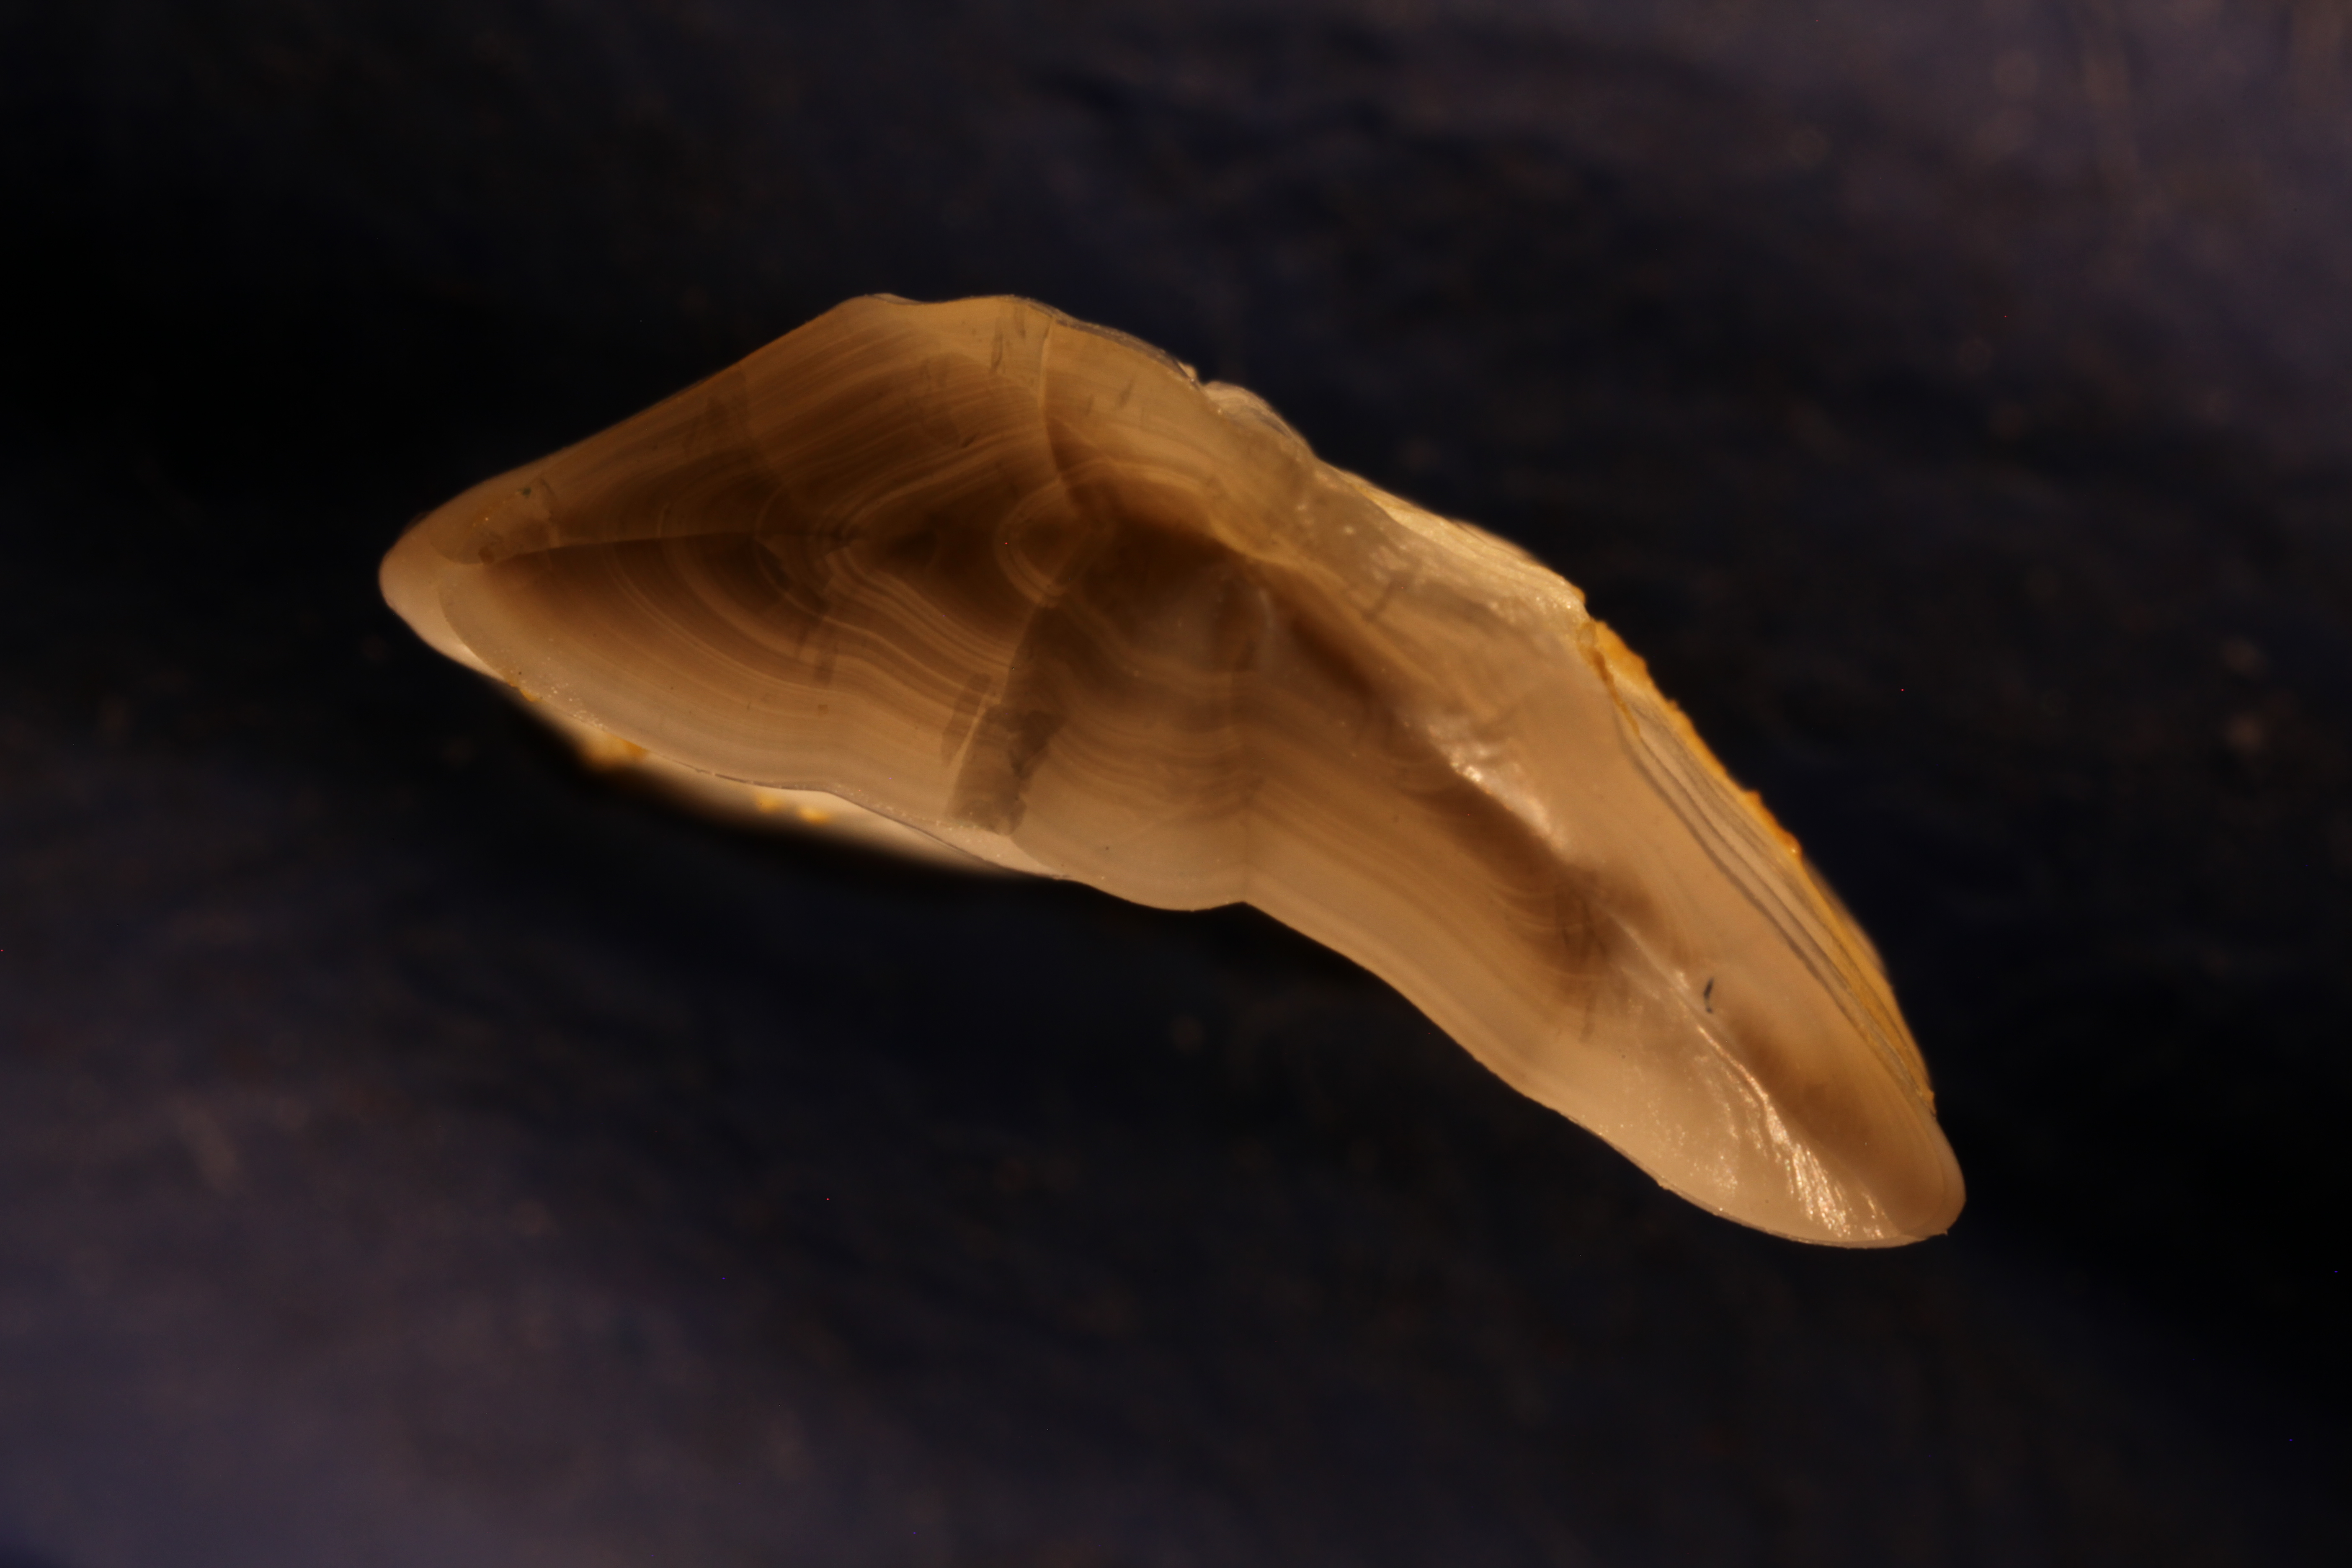
\includegraphics[scale=0.015]{otolith/IMG_0457_2016_70021.JPG}
  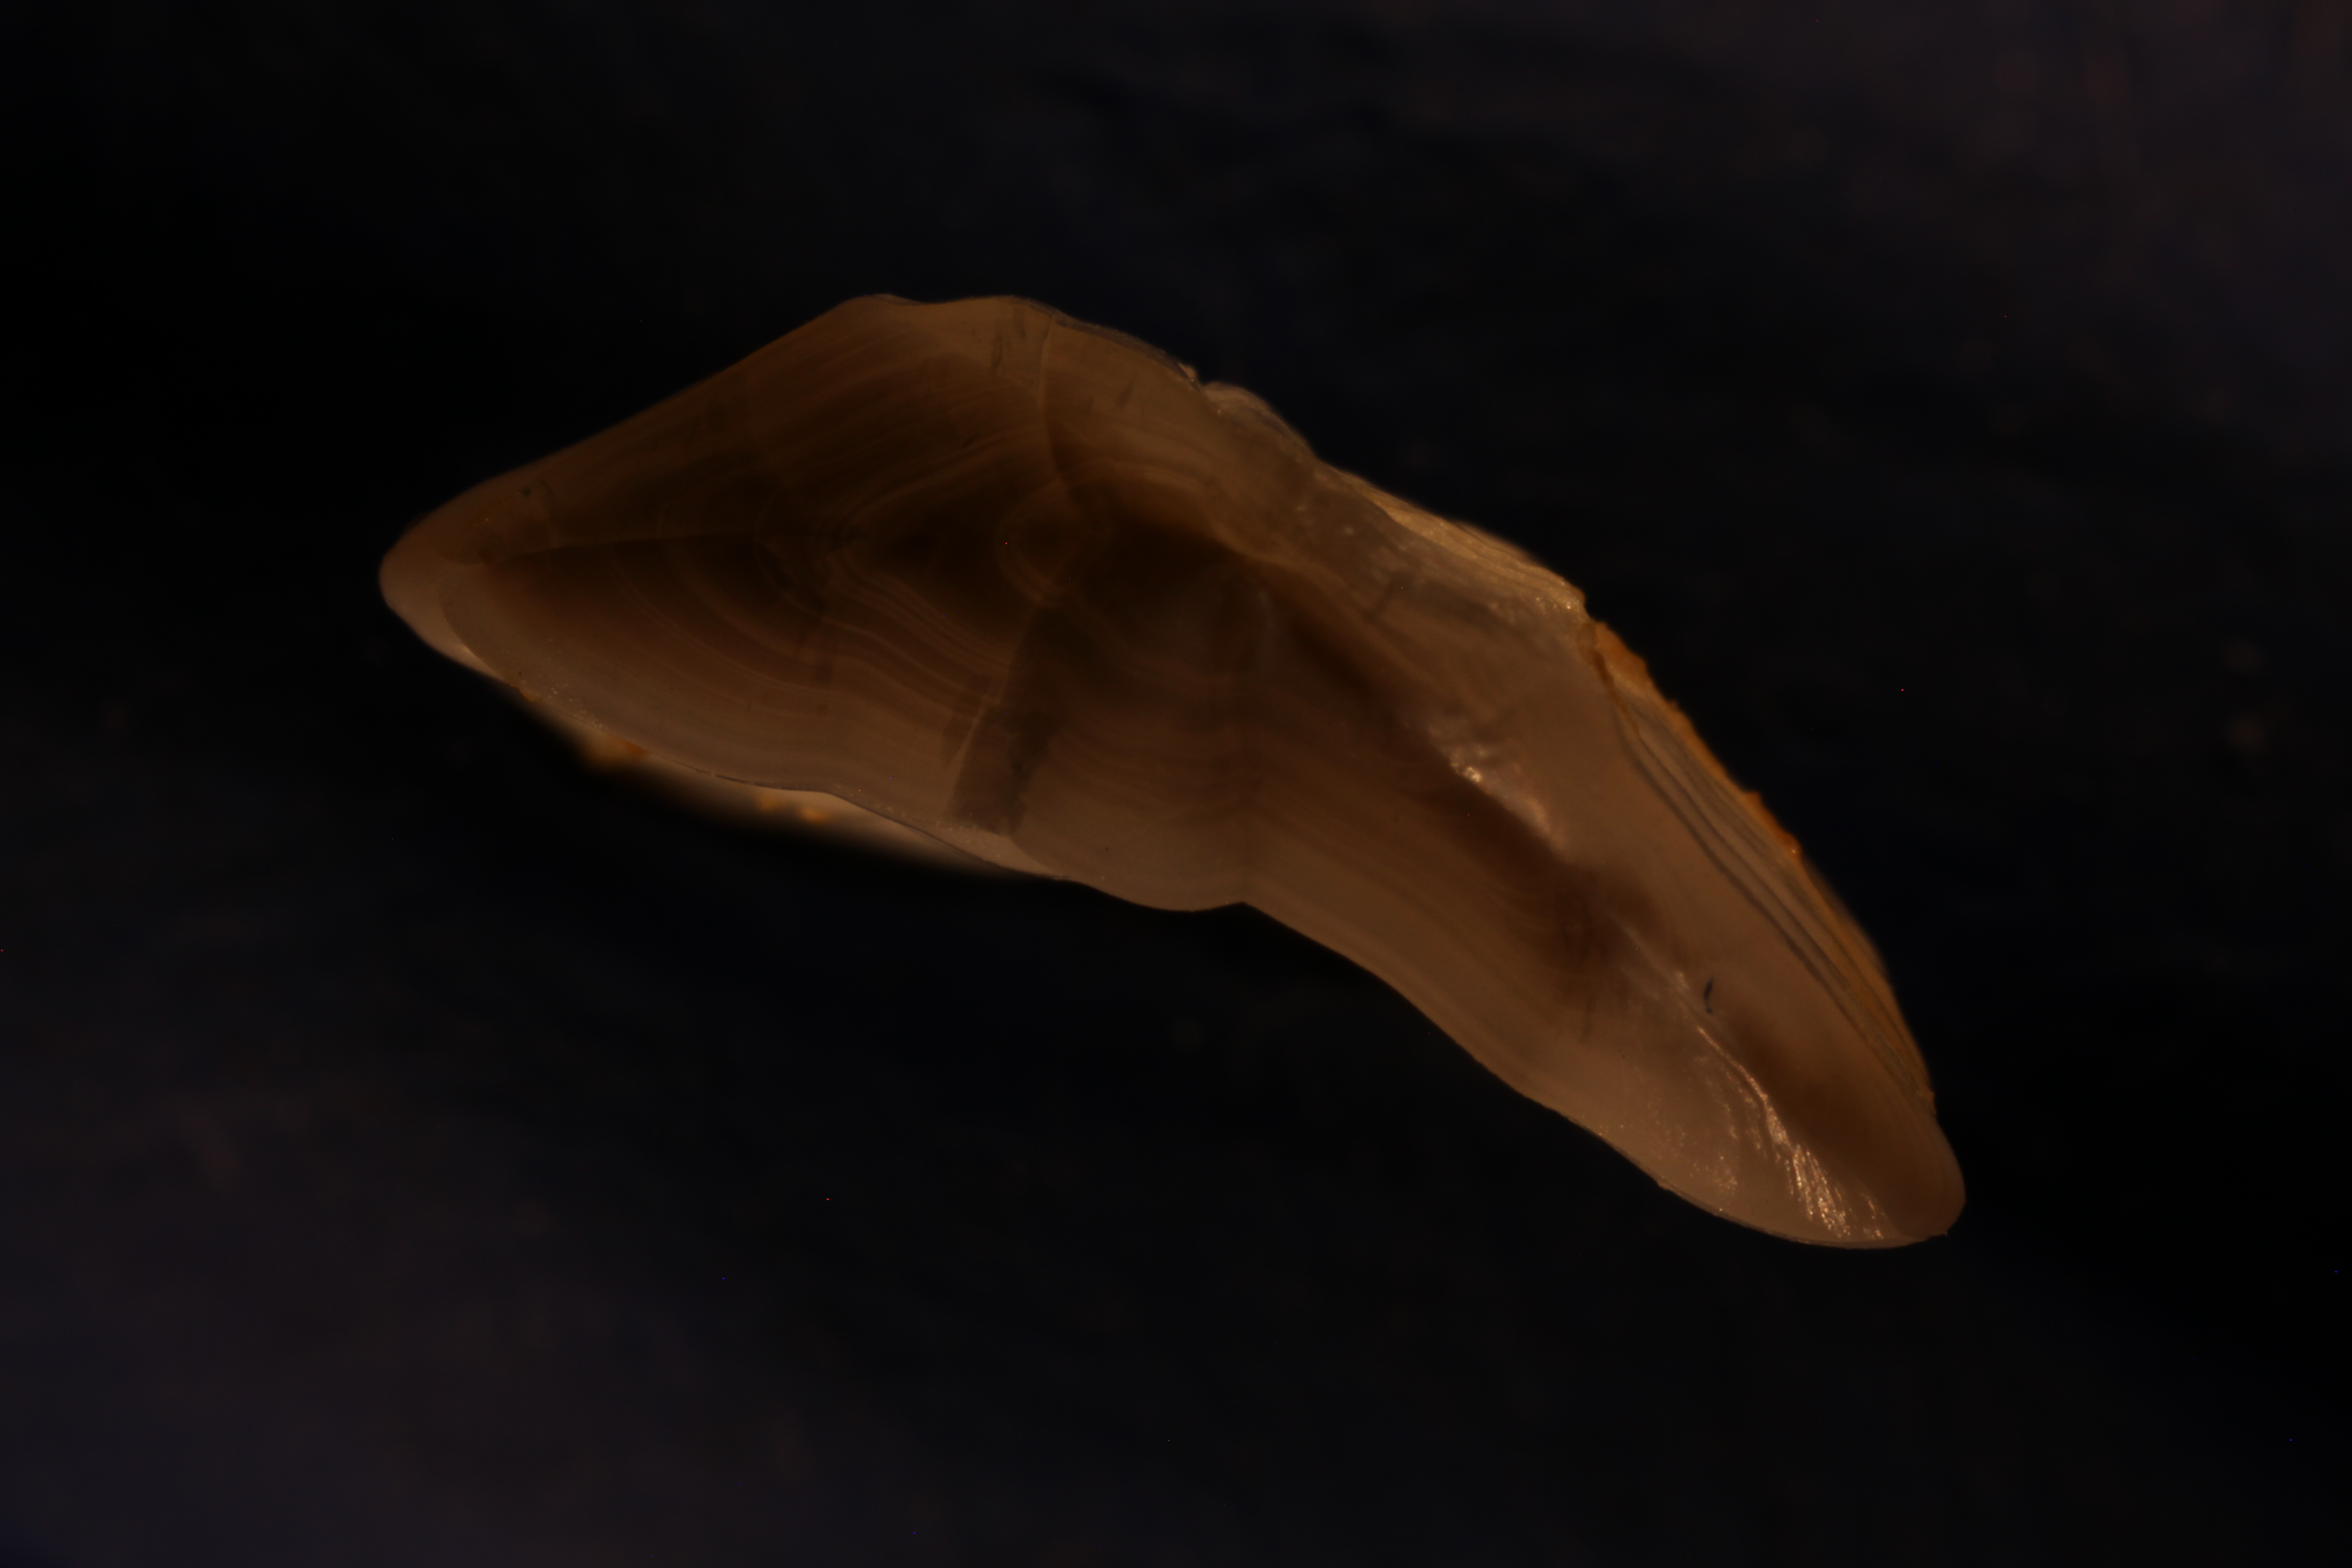
\includegraphics[scale=0.015]{otolith/IMG_0458_2016_70021.JPG}
  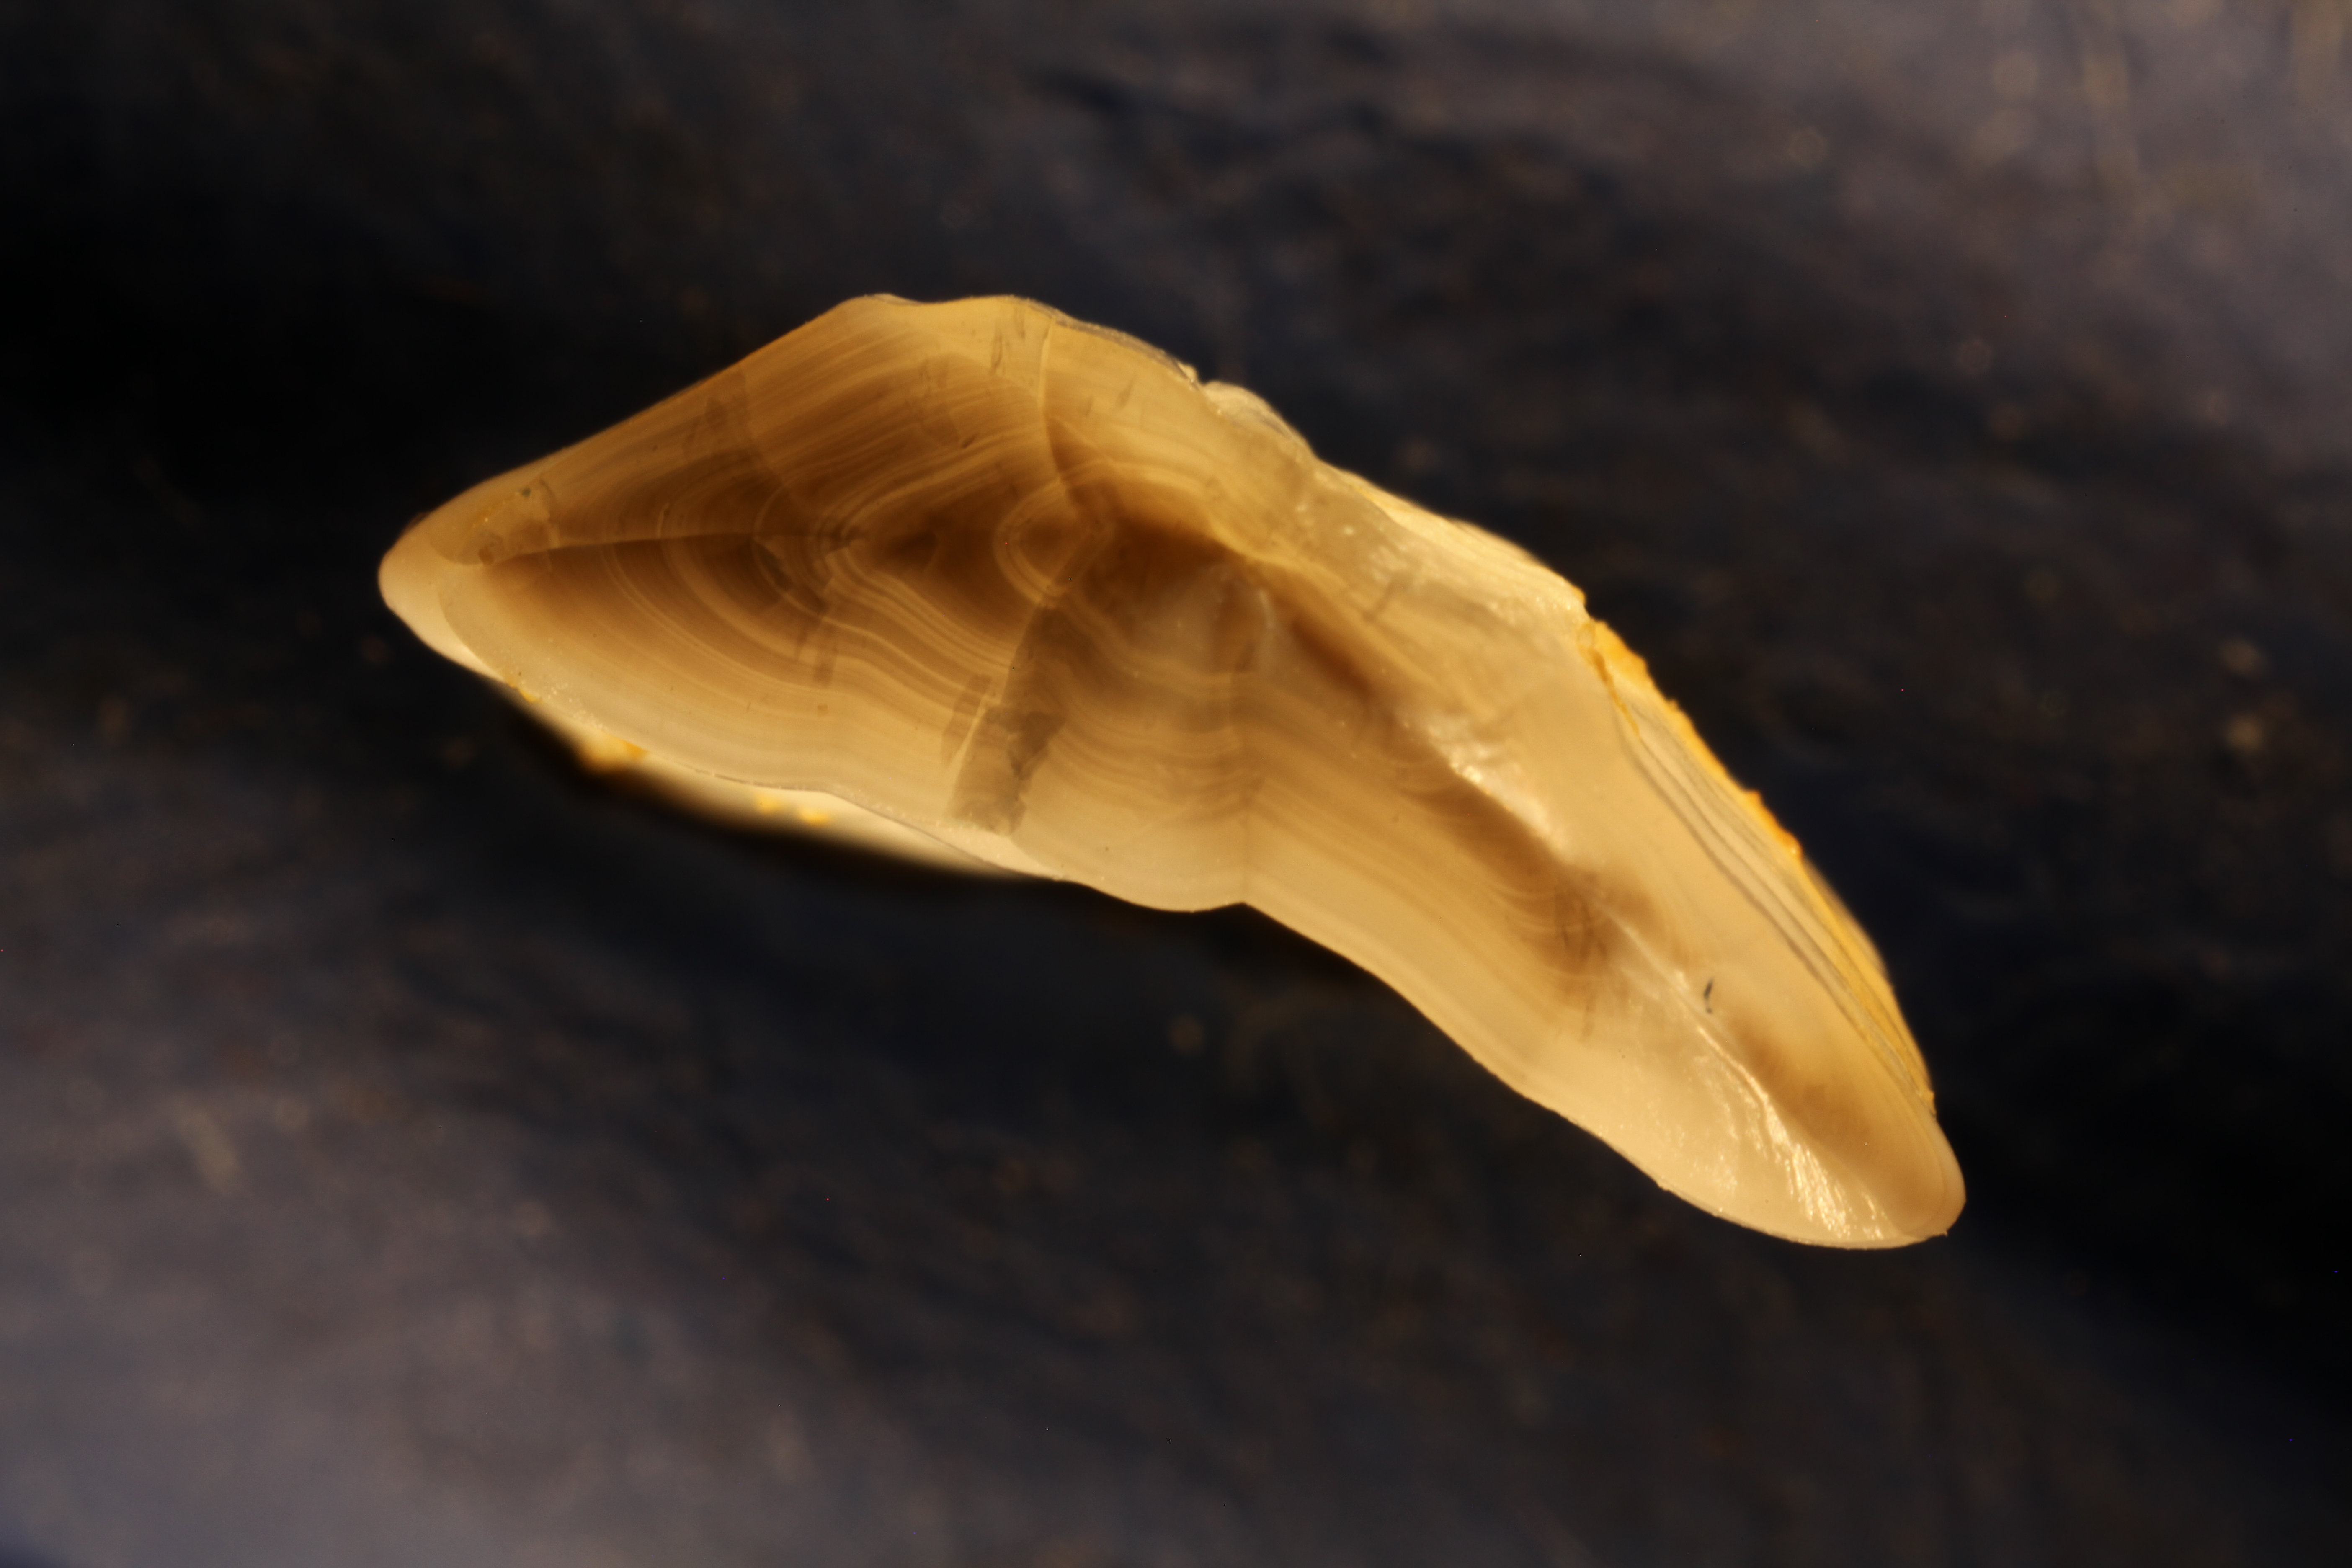
\includegraphics[scale=0.015]{otolith/IMG_0459_2016_70021.JPG} 

  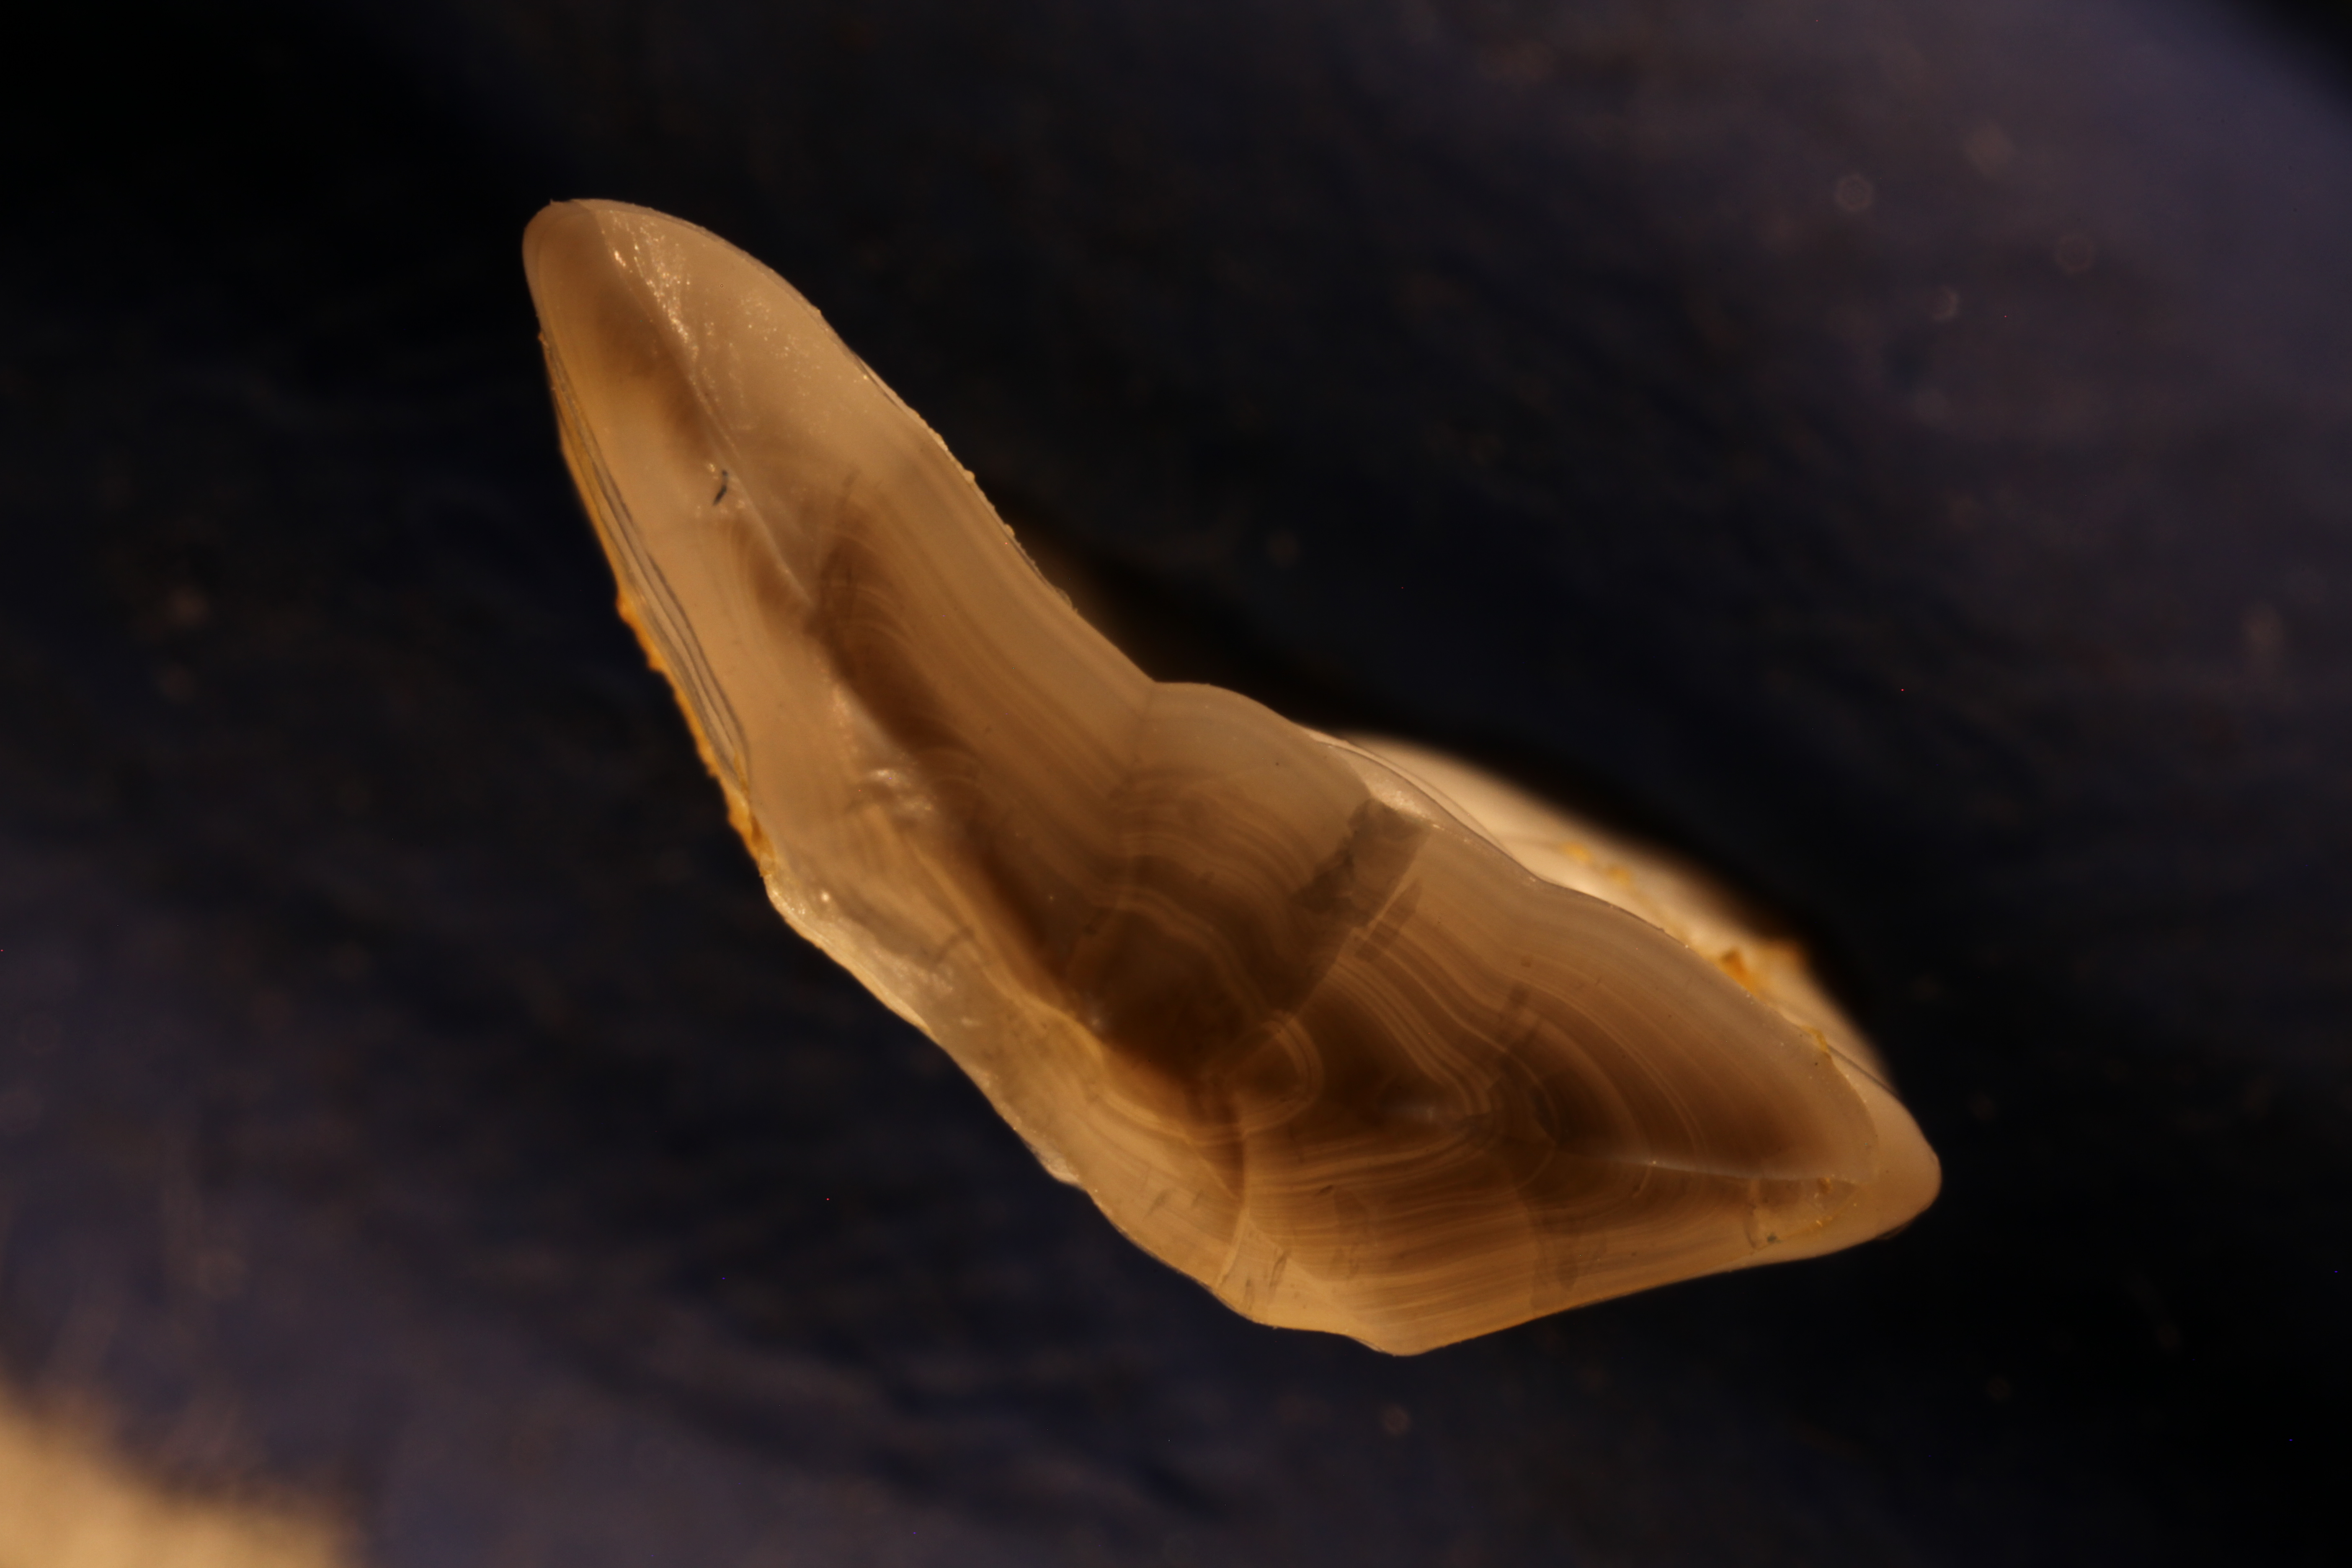
\includegraphics[scale=0.015]{otolith/IMG_0460_2016_70021.JPG}
  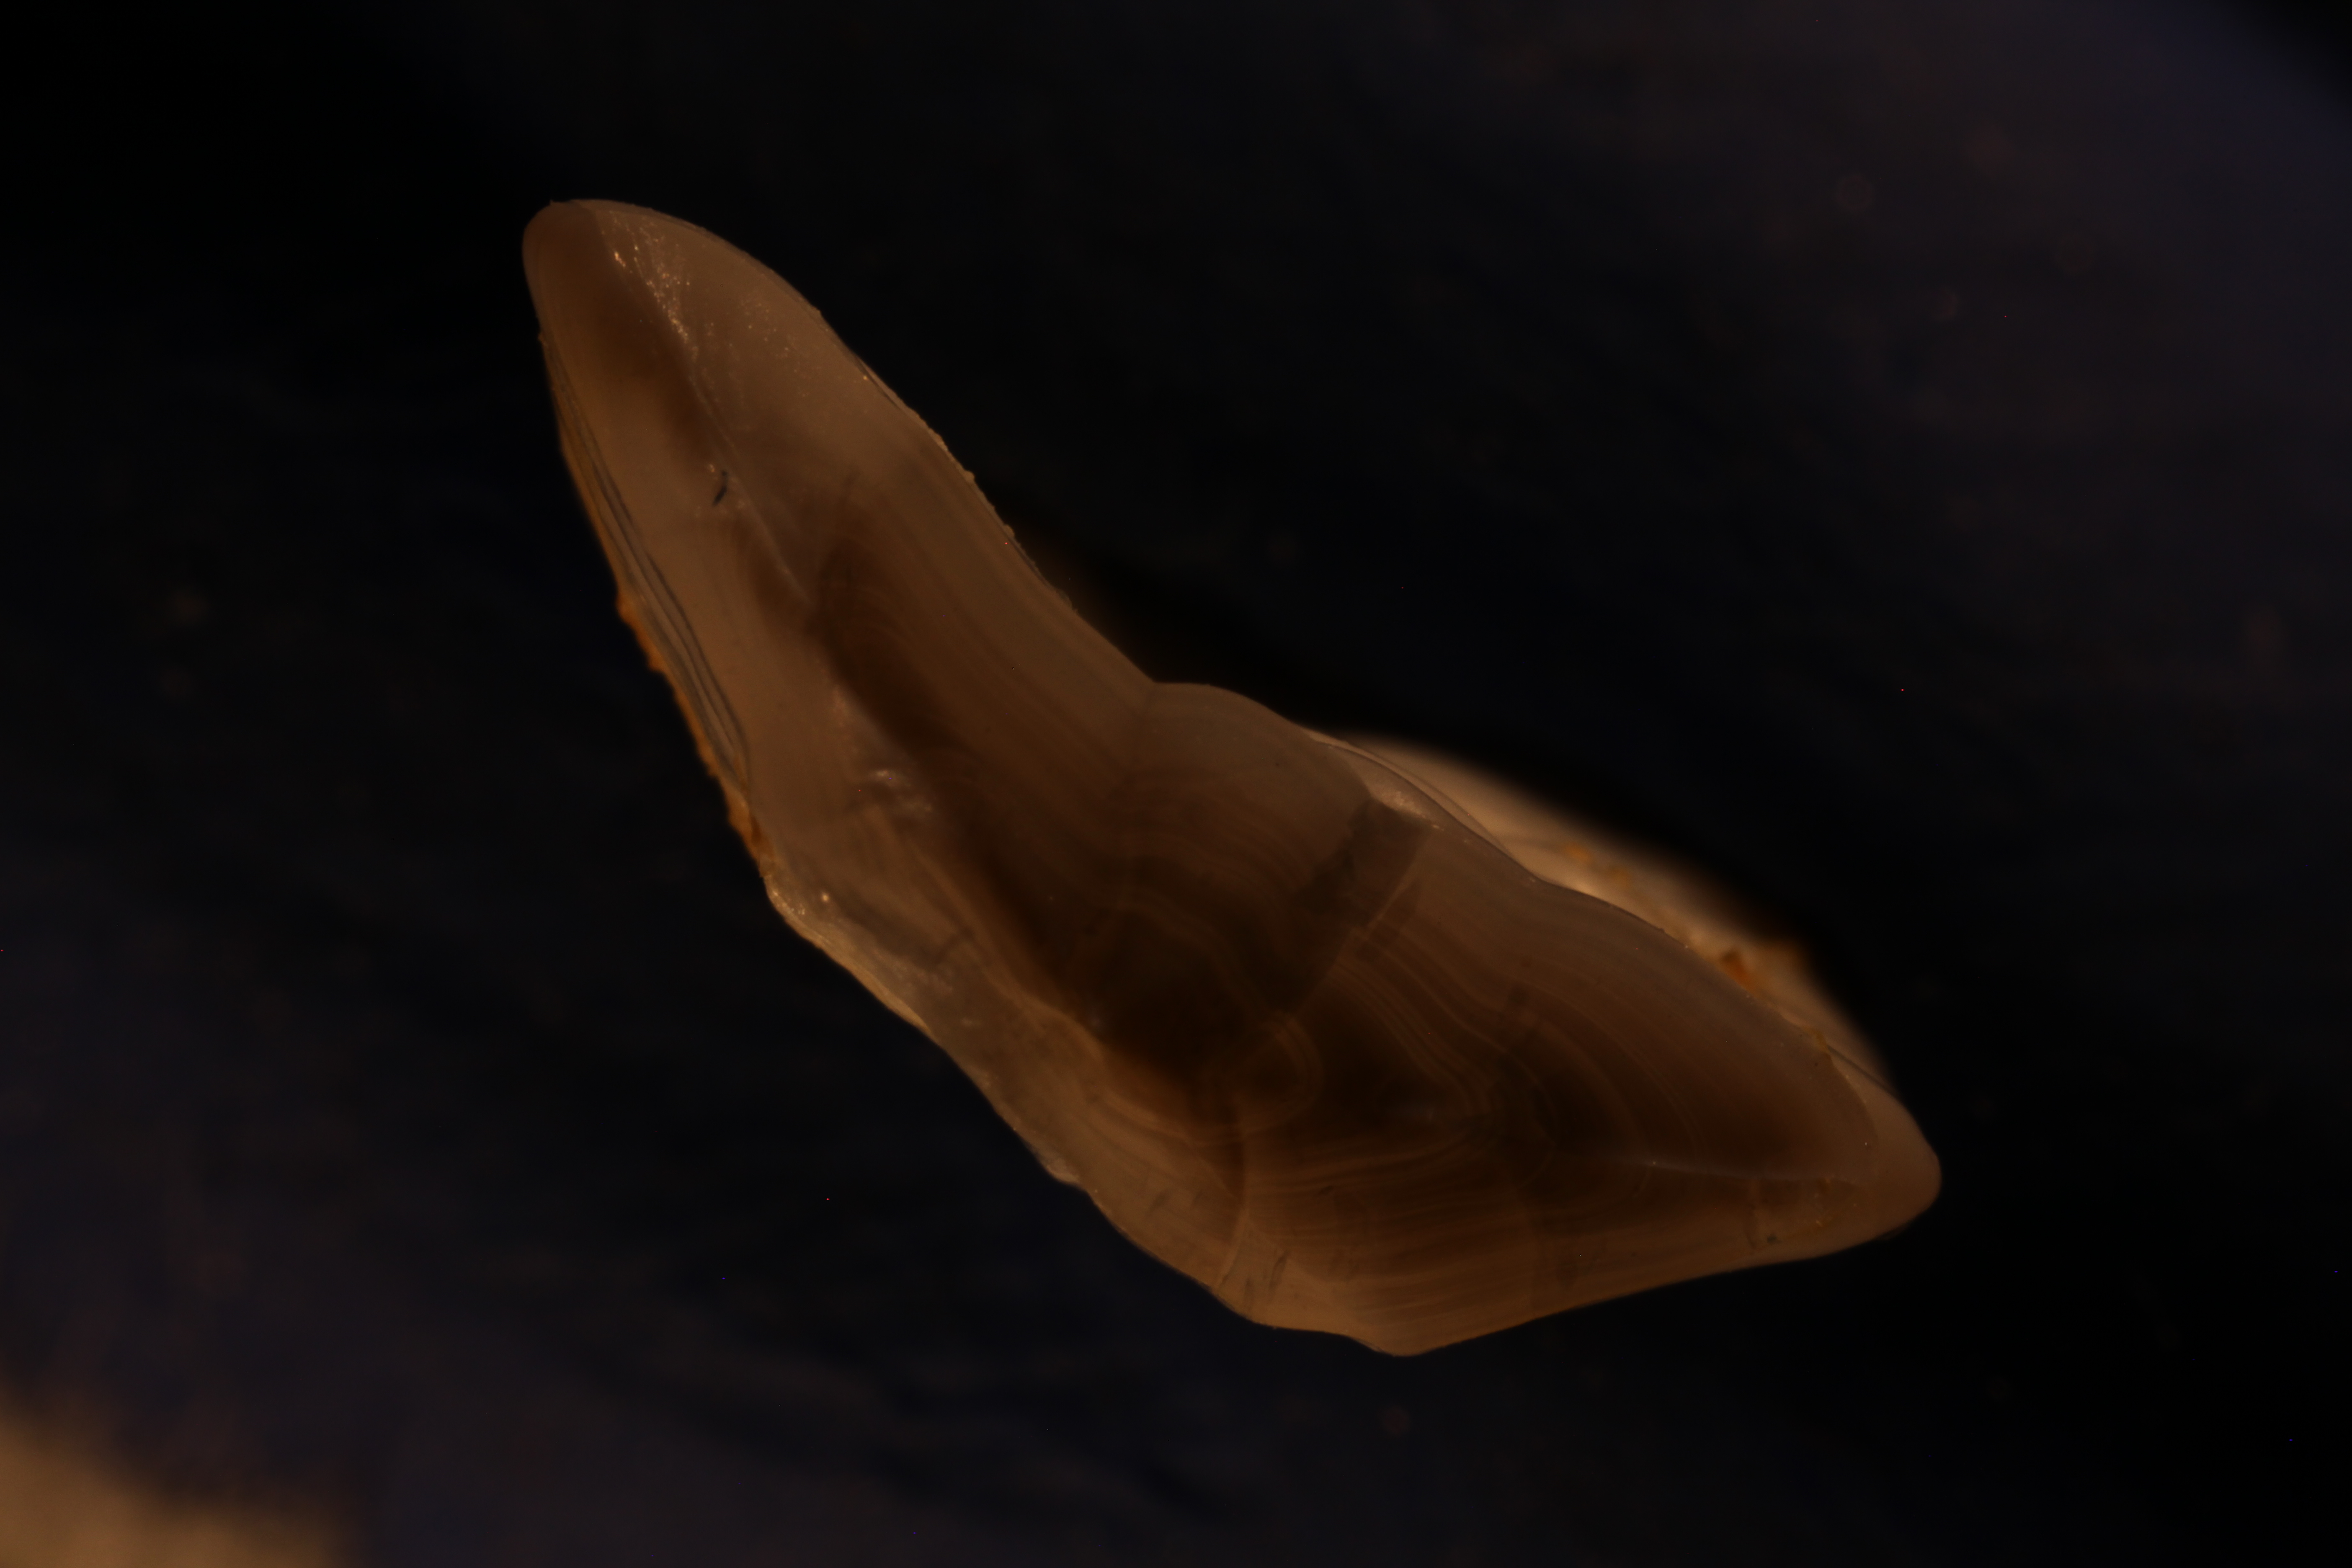
\includegraphics[scale=0.015]{otolith/IMG_0461_2016_70021.JPG}
  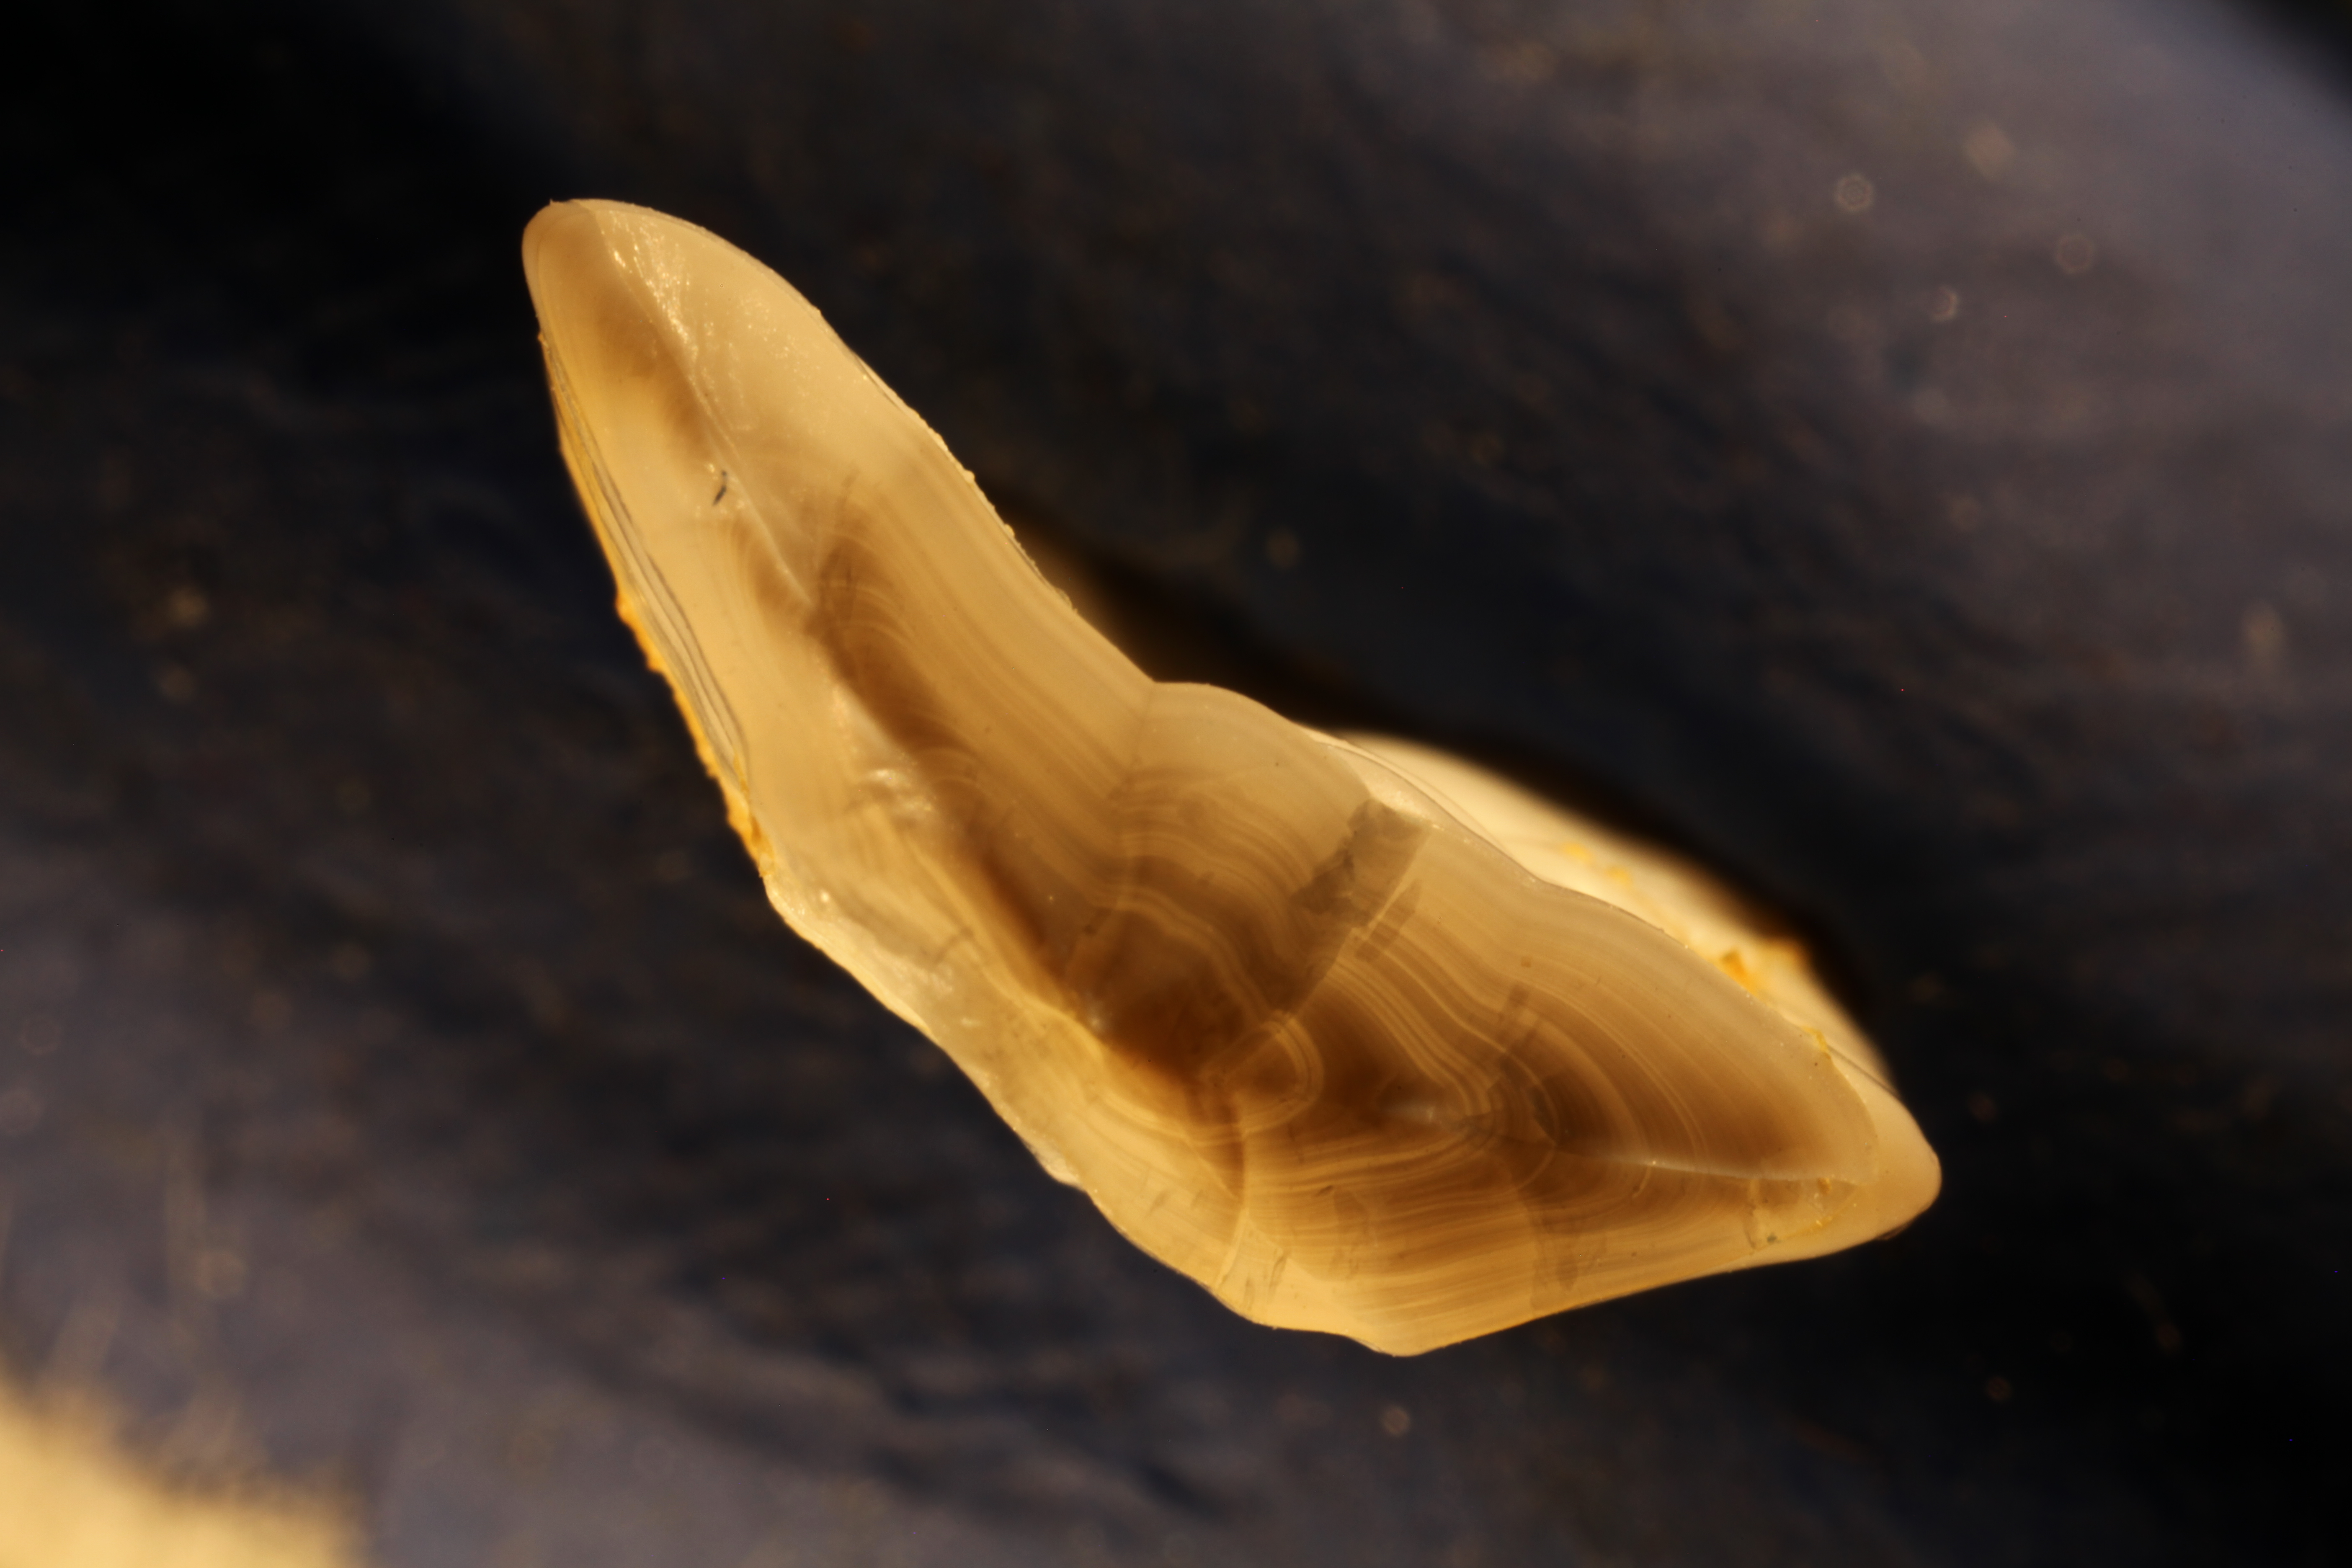
\includegraphics[scale=0.015]{otolith/IMG_0462_2016_70021.JPG}
  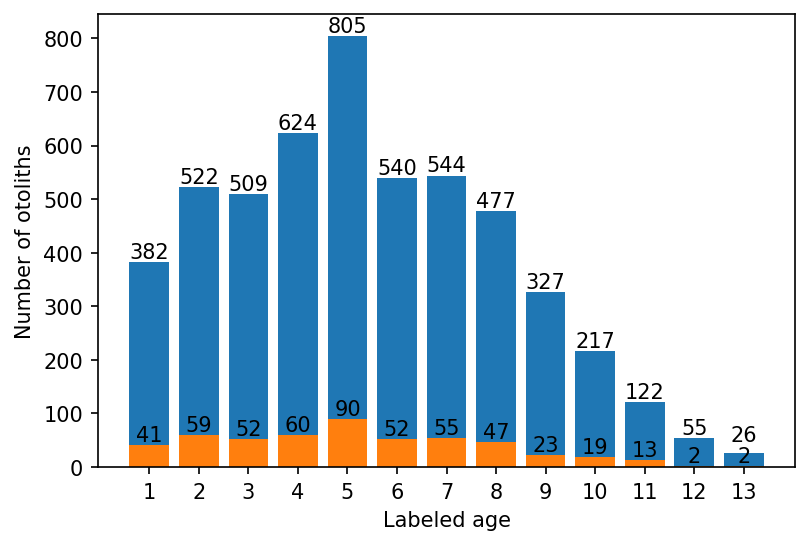
\includegraphics[scale=0.8]{distribution/age_dist_all_test.png}
    \caption{Images of an otolith collected in 2016 from a 6 years old cod (top), taken with medium-, minimum- and max-exposures (upper row), then rotated 180° (lower row). The age distribution of the 5150 otoliths in the training (blue), and the 515 otoliths in the test (orange) set (bottom).}
  \label{marker1}
\end{figure}

\subsection{Convolutional neural network architecture}


Each CNN was trained using transfer learning by loading ImageNet weights. The training images were resized from 3744$\times$5616 pixels to between 380$\times$380 and 528$\times$528 pixels
depending on the architecture. The pixel values have a range between 0 and 255, which was normalized to between 0 and 1. Test set predictions were done on images resized to 380$\times$380 and 384$\times$384 pixels. To investigate the effect of exposure and orientation as presented in the image-taking protocol described in \citep{codOtolithsMyers}, we also trained on 9-channel images by stacking the three color layers from each of the threeimages representing different lighting exposures. Using Timm \citep{rw2019timm}, the ImageNet weights were duplicated on the input layer to accommodate all 9 channels. The three images used were of dark, medium, and light exposure. 

CNNs were selected based on performance on the ImageNet benchmark and the availability of open-source implementations with pre-trained weights. The CNN models are aimed at classification, while we treated aging as a regression problem \citep{moenetal, vaboeetal}. The last layer of the CNNs was therefore modified to  a linear output. For the EfficientNetV2 family we did this by applying three multi-layer perceptron layers going from 1280 output of the last hidden layer to a dense 256-layer, 
then a leakyRelu \citep{DBLP:journals/corr/XuWCL15} layer, then a dense 32-layer, then a leakyRelu layer, and finally a linear output layer. For EfficientNet we only changed the last layer from softmax to a linear output (Figure \ref{fig99} in supplementary materials).

To each fold, we normalized the age on the training set by subtracting the mean and scaling to unit variance. The normalization was then applied to the validation and test sets. Test set predictions were obtained by applying the inverse transform.

\subsection{Implementation and training}

EfficientNetV1 B4, B5, and B6 were imported and modified with TensorFlow \citep{abadi2016tensorflow} and Keras \citep{keras} software packages in Python. Computation was done using CUDA 11.1 and CuDNN with Nvidia (Nvidia Corp., Santa Clara, California) A6000 accelerator card with 48 GB of GPU memory and P100 cards with 12 GB of GPU memory,
EfficientNetV2 Medium, and Large were imported and modified with the PyTorch \citep{NEURIPS2019_9015}  and Timm \citep{rw2019timm} software packages. Computation was done on P100 and RTX 3090 with 24 GB of GPU memory. Pretrained weights for EfficientNet were available from Keras, and pre-trained weights for EfficientNetV2 were available from Timm. The models will be referred to as B4-Min, B4-Middle, B4-Max, B5-Min, Medium-min and so on by combining model name with image exposure.

Augmentation is a commonly used technique to artificiallly inflate the training data set by applying transforms that modify the input while preserving class. The images were augmented using rotation between 0 and 360 degrees, and reflection by the vertical axis. 

The cost function used was mean squared error (MSE)
while the metric used for evaluating the models and comparing them to expert readers was accuracy. Accuracy was obtained by rounding the real valued predictions to the nearest integer and measuring the fraction of otoliths where the age classification matches the labels.

% k-fold cross validation
The data set of 5150 otoliths was divided into a training set constituting 90\% of the otolith images (4635 otoliths) and a test set of 10\% (515 otoliths).
To get the most out of a small data set we applied 10-fold cross-validation on the training set. The data set is divided into ten parts, and in each iteration (or "fold"), a different part is retained for validation, while the model is trained on the remaining nine parts. In other words, 10 different models were trained with a different set of 463 images used for validation in each fold, i.e. each data point participates in the validation set once and in the training set 9 times. Among the 10-fold models, the one with the best MSE was chosen. The best model parameters on the validation set were then used to predict the age on the test set, and the metric for accuracy and MSE were recorded. The test set is chosen at random, while the 10-fold split of the training set is chosen using a stratified k-fold split, which preserves a similar distribution of the whole cross-validation set in each validation set. That means the 463 images in the validation set will have similar age distribution to that of the 4635 images in the cross-validation set. 

\subsection{Hyper-parameters}

The CNN hyper-parameters (i.e., model parameters that are set in advance, in contrast to model parameters that are learnded during training) configurations varied a little between the two families of networks, but were kept the same within the families. Some hyper-parameters that were tuned are batch size, learning rate, k-fold size, weight decay, step size, number of epochs, early stopping, and patience. Some parameters are constrained by the GPU memory, like batch size which
was set to 16 for models trained on the A6000 card, and to 8 for the models trained on P100s.

EfficientNet used learning-rate with a weight decay scheduler, while EfficientNetV2 
used Cosine Annealing scheduler \citep{Loshchilovetal}. The training- and validation 
image size used was not changed, except for EfficientNetV2 Large which uses a smaller validation image size. The exact configuration of each network is available with each network result on the GitHub page of the project (https://github.com/emoen/Deep-learning-for-regression-of-cod-otoliths). The hyper-parameters are available in Table \ref{table2}, and \ref{table3} in supplementary information.

\subsection{Ensemble learning with averaging}

Ensemble learning is an algorithm that combines the predictions from multiple models to reach a final prediction and obtains a predictive performance that is better than any of the constituent models alone.

We evaluated two types of simple ensemble averages. The first ensemble was the average of the 10-fold cross-validation, which was reported as the model performance. This ensemble of 10 model weights was reported as one model because the architecture and image exposure was the same. Only the training and validation data were different in these models. The model weights were selected during training when the model had the lowest MSE on the validation set. The average MSE and accuracy of the prediction of the 515 test images from 10 folds on the test set were reported as the model MSE, and accuracy.

The second ensemble was created from selections consisting of 2, 3, 4 models, and so on up to an ensemble containing all 17 models. These ensembles combine 20, 30 and up to 170 predictions on the test set. The accuracy was reported after rounding. 

\subsection{Correlations of predictions on the test set and clustering analysis}

Correlations of predictions on the test set were investigated by creating a correlation matrix of each model's prediction of each age class. This matrix showed how much the models were in agreement, and clustering analysis identified which models were more in agreement with each other.  We used Pearson's correlation coefficient and hierarchical clustering (HCA) with Euclidean distance and complete linkage. 

\subsection{Comparison of CNN with human readers}
To evaluate the credibility of CNN predictions in relation to human readers, we compared the mean percentage agreement of the test set predictions within each age class with those from multiple human readers from a recent internal cod age reading workshop carried out in 2021 at the Institute of Marine Research, Norway. In this workshop, a set of 100 broken otoliths from Atlantic cod were read by seven readers, of which five were certified advanced cod readers and two were under training. By comparing the results of the test set to the mean agreement and standard deviation of predictions within the age class from the workshop, we evaluated if machine-driven estimates were behaving in line with those anticipated by human readers.

\section{Results}

The mean accuracy of the 17 models was 72.7\% (Table \ref{table4}) on the test-set, and 
the standard deviation was 1.1.
The least accurate model was B4-max with 70.9\%, and the most
accurate model was B5-min and B6-middle with an accuracy of 74.4\%.


B5 was the highest scoring model on all the exposures (min, middle, max) with a mean accuracy of 73.7\%,
and min-exposure was the best exposure with a mean accuracy of 73.3\%
Both B5 and B6 from the EfficientNet family were better than 
Medium and Large from the EfficientNetV2 family.

\begin{table}[hbt!]
\caption{Mean accuracy, MSE, and Percentage Agreement (PA) on the test-set by light exposure and CNN architectures}
\begin{tabular}{ |l|c|c|c|c|c|c|c|} \hline
    & \multicolumn{3}{|c|}{EfficientNet V1} & \multicolumn{3}{|c|}{EfficientNet V2} \\ \hline
    Acc:light/CNN & B4 & B5 & B6 & Medium & Large & Mean \\ \hline
    min        & 72.8 & {\bf 74.4} & 73.4      & 74.0 & 72.0 & 73.3 \\ 
    middle     & 71.5 & 73.4        & {\bf 74.4} & 72.4 & 72.8 & 72.9 \\ 
    max        & 70.9 & 73.2        & 71.5       & 71.3 & 72.4 & 71.9 \\ 
    9 channels & -    & -           & -          & 74.0 & 72.2 & 73.1 \\  \hline
    {\bf Mean} & {\bf 71.7} & {\bf 73.7}     & {\bf 73.1}  & {\bf 72.9} & {\bf 72.4} & {\bf 72.7} \\  \hline
    MSE:light/CNN &  &    &       &  &  &  \\ \hline
    min        & .277 & .277 & .272      & .273 & .280  & .276 \\ 
    middle     & .285 & .273 & {\bf.262} & .278 & .275  & .275 \\ 
    max        & .291 & .359 & .305      & .289 & .286  & .306 \\ 
    9 channels & -    & -    & -         & .273 & .271  & .272 \\ \hline
    {\bf Mean}       & {\bf.284} & {\bf.303} & {\bf.280}  & {\bf.278} & {\bf.278}  & {\bf.284} \\ \hline
    PA:light/CNN &    &    &    &      &  &  \\ \hline
    min          & 89.5 & 89.3 & 88.2 & 89.7       & 89.9 & 89.3 \\ 
    middle       & 88.2 & 89.5 & 90.9 & 91.1       & 87.8 & 89.5 \\ 
    max          & 87.6 & 90.5 & 88.0 & 89.5       & 90.3 & 89.2 \\ 
    9 channels   & -    & -     & -   & {\bf91.3} & 91.1 & 91.2 \\ \hline
    {\bf Mean}   & {\bf 88.1} & {\bf 89.8} & {\bf 89.0} & {\bf 90.4} & {\bf 89.8} & {\bf 89.6}  \\ \hline    
\end{tabular}
\label{table4}
\end{table}
The mean MSE of the 17 models was 0.284 on the test set, and the standard deviation was 0.022.
The highest MSE was from B5-max with MSE of 0.359, and the lowest MSE was from B6-middle exposure with MSE of 0.262.
We find that the differences between models were statistically significant (ANOVA, p = $1.6 *10^{-7}$), but that the differences were not significant for the individual factors of model architecture (two-way ANOVA, p = 0.139) or image exposure (p = 0.057). See Table \ref{table5c} in the supplementary information for a T-test of all models.  From the interaction plot for two-way ANOVA, we see that using low exposure images is more beneficial for the smaller models (Figure \ref{marker20}).

\begin{figure}[htpb!]
\centering
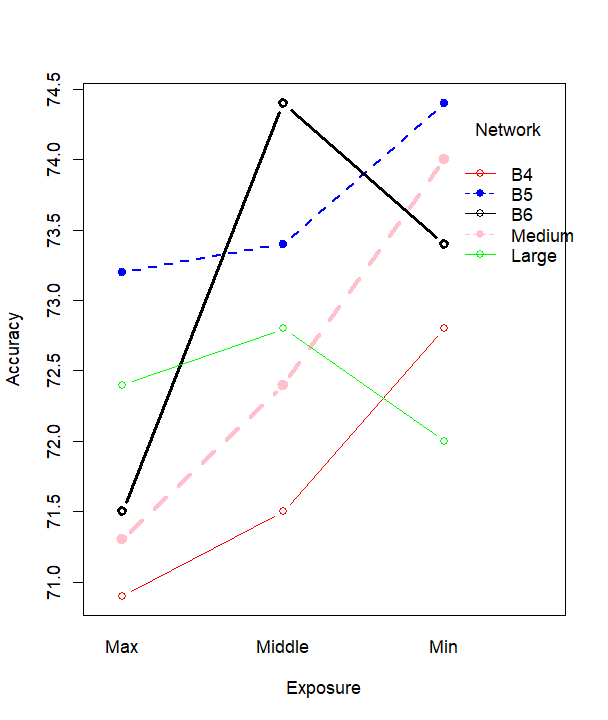
\includegraphics[height=1.0\textwidth, width=1.0\textwidth]{results/eda/interactive_two_way_anova_exposure.png}
  \caption{Interaction plot of the 5 networks
  with image exposure on x-axis and 
  ensemble accuracy on the y-axis. We
  see that under-exposed images perform
  better for all but the B6 and Large network.}
  \label{marker20}
\end{figure}

Medium and Large were the best models with a MSE of 0.278,
and the 9-channel composite images gave better results than any individual exposure, with a MSE of 0.272.
The high MSE for B5-max and B6-max was due to a large misprediction of the image with index 308 in the test set labeled 1 year and predicted 5.7 years (see Table \ref{table10} in supplementary information on outliers).

Medium-all was the highest scoring model with percentage agreement (PA) 91.3\% and B4-max was the lowest scoring model with PA 87.6\% (Table {\ref{table4}}). Medium was the overall best performing model and B4 was the worst. The 9-channel composite images outperformed individual exposures, while max exposure had inferior performance to the others.

When comparing each 10-fold ensemble average prediction accuracy, and MSE for all 17 models, 
the ensemble metric was either better than or in the upper quantile for all the models (Figure \ref{marker10}). The prediction MSE and accuracy of each fold are given in supplementary information (Table \ref{table11}, \ref{table12}).

\begin{figure}[htp!]
\centering
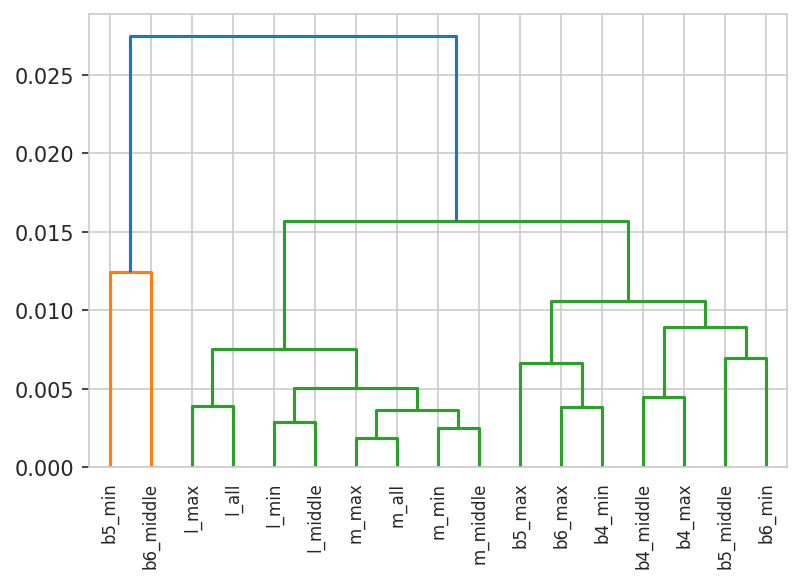
\includegraphics[height=60mm,width=0.8\textwidth]{results/eda/hca.png}
\includegraphics[height=70mm,width=0.8\textwidth]{results/eda/box_plot_models_acc3_yaxis.png}
\includegraphics[height=70mm,width=0.8\textwidth]{results/eda/box_plot_models_mse3_yaxis.png}
    \caption{Hierarchical clustering (HCA) on the correlation of predictions (top), a box-plot of accuracy score (middle), and MSE (bottom) of all the 17 models. In (middle) and (bottom), the blue line is ensemble-average prediction accuracy (or MSE) on the test set, the red lines are the two best ensemble-average predictions on the accuracy, and the orange lines are the mean of the 10-fold predictions.}
  \label{marker10}
\end{figure}

\subsection{Prediction by age class}

When calculating the accuracy of all models by age class, we found that accuracy for one- and two-year-olds was better than 90\% 
(supplementary information in Figure \ref{marker6}).
All age classes six years or younger were correctly classified with more than 70\% accuracy, and all 13-year-olds were predicted to be younger.

No systematic bias in the age prediction of CNN is visible except for the underestimated age of individuals aged by the expert reader as 13 years old (Figure \ref{marker7}).

\begin{figure}[hbt!]
  \centering
  \centering
  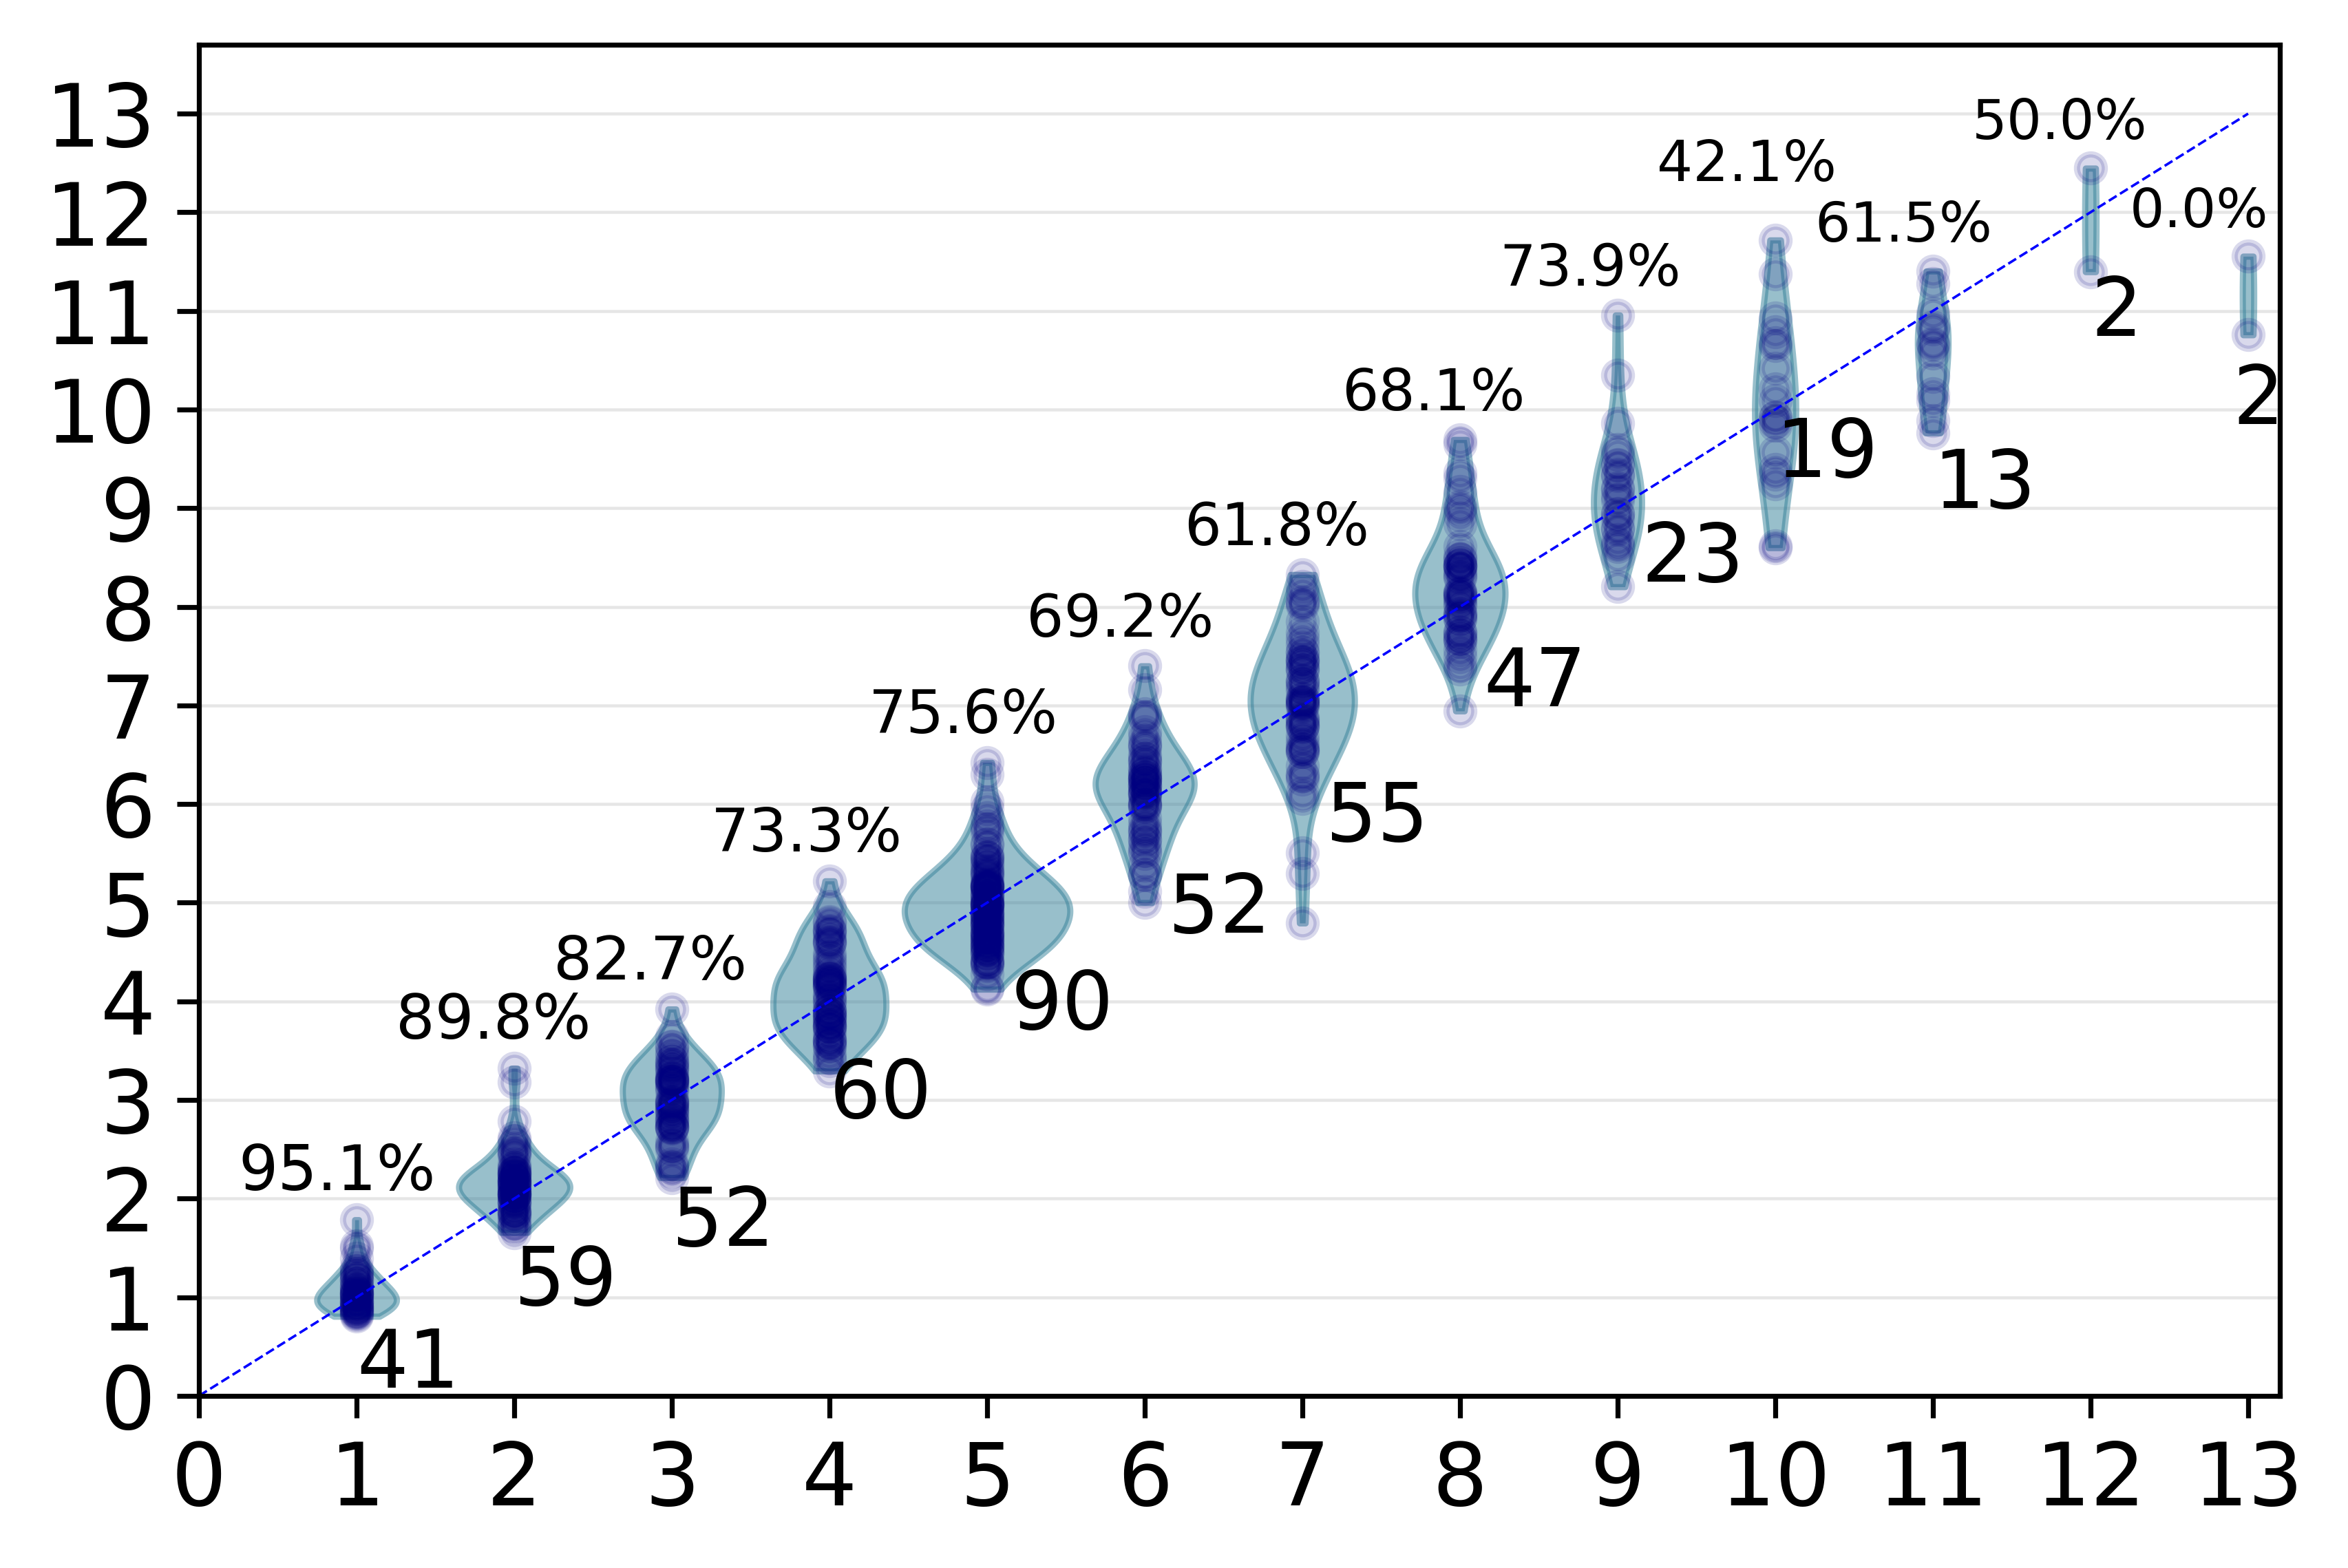
\includegraphics[scale=0.33]{results/eda/violin_plot_age.png}
    \caption{Violin plot of predicted age from model B5-min with accuracy of 74.4\%. 
  Above each age is the accuracy, and below is the total number of images 
  in the test set of that age class}
    \label{marker7}
\end{figure}


\subsection{Simple ensemble-average predictions}

We searched the space of ensembles-average predictions
of 2 to 17 models, which is the set of unordered combinations without replacement,
equal to the binomial coefficient 
$\sum_{k=1}^{N}\binom{N}{k} $ where $N=17$ and $k \in 2.N$
For each set of ensemble combinations, we recorded the best 
ensemble and found that the best overall ensemble prediction 
was an ensemble of six models which produced an accuracy of 78.6\%. 
The ensemble consisted of B4-min, B5-min, B6-min, Medium-min, B6-middle, and B4-max.
The results are presented in detail in supplementary information in Table \ref{table6}, \ref{table7}, and \ref{table9}.

The ensemble accuracy decreased after adding 6 models, while the
MSE continued to decrease until all 17 models were included.
This was as expected from the theory on simple ensemble average learning
since the variance is reduced with more models.

\begin{center}
\begin{table}[hbt!]
\caption{Rank statistics of models by participation in the best ensemble of size 1 to 17 when the loss function is accuracy.}
\begin{tabular}{ |l|l|l| }
\hline
Rank & Model name & Count   \\ \hline
1 &  B4\_min & 15 \\ \hline
1 &  B6\_min & 15 \\ \hline
3 &  B5\_min & 13 \\ \hline
3 &  M\_min  & 13 \\ \hline
5 &  B6\_mid & 12 \\ \hline
6 &  B5\_mid & 10 \\ \hline
6 &  B4\_max & 10 \\ \hline
8 &  L\_mid  & 9 \\ \hline
9 &  B6\_max & 8 \\ \hline
10 & M\_mid  & 7 \\ \hline
10 & M\_all  & 7 \\ \hline
10 & L\_all  & 7 \\ \hline
13 & M\_max  & 6 \\ \hline
14 & L\_min  & 5 \\ \hline
14 & B4\_mid & 5 \\ \hline
14 & B5\_max & 5 \\ \hline
14 & L\_max  & 5 \\ \hline
\end{tabular}
\label{table8}
\end{table}
\end{center}

We observe that the models B4-min (No 1) and B6-min (No 3) were the most often present in the top scoring model with inclusion in 14 ensembles (Table \ref{table8}). These models did not have the highest accuracy (B5-min, and B6-middle) but an accuracy of 72.8\% and 73.4\%. This was lower than the highest accuracy models, which were B5-min and B6-middle (74.6\%) with a rank of 3 and 5, respectively.

The mean ranking by exposure types was: min-exposure (rank 4.4), middle-exposure (rank 8.6), 9-channel composite (rank 10), and max-exposure (rank 11.2). The mean ranking by architecture was EfficientNet (rank 6.6), and EfficientNetV2 (rank 10.3).

\subsection{Outliers}

Figure \ref{marker8} shows 4 images that were incorrectly classified with an error larger than 1 year after rounding. All the images with more than 1 year in prediction error are shown in supplementary information (Table \ref{table10}), with comments by an expert on the most
common mispredictions (Table \ref{table10b}). Large outliers occurred throughout all of the tested models and ensembles in small numbers. Most of those outliers were identified as visually challenging images with artifacts and/or low readability. For example, image 13 was overestimated in all B models, likely due to a clear zone in the inner core region that an expert reader would identify as a settlement false zone and ignore. Similarly, many outliers, such as images 270 and 369, showed multiple narrow false zones in the mid-section of the otolith that were likely to affect age determination. Alternatively, cases such as images 71 and 342 showed clear issues with age interpretation when the image deviates from the standard of the training set, such as when the exposure was changed drastically or when break lines interrupted the normal pattern of ring deposition. In one case (image 362), all models estimated the otolith to be 5 instead of 7 years old: upon visual investigation, the otolith was clearly 5 years old, and the initial age had likely been misread.

\begin{figure}[hbt!]
  \centering
  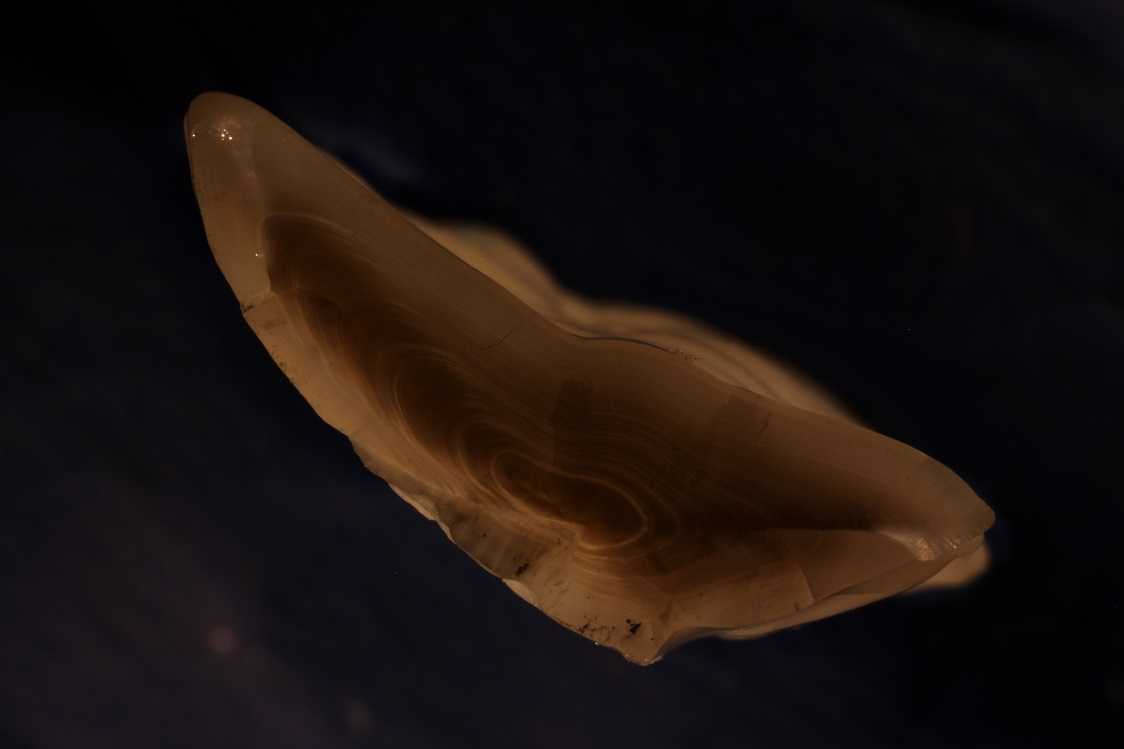
\includegraphics[width=0.45\textwidth]{outliers/IMG_0284_13.JPG}
  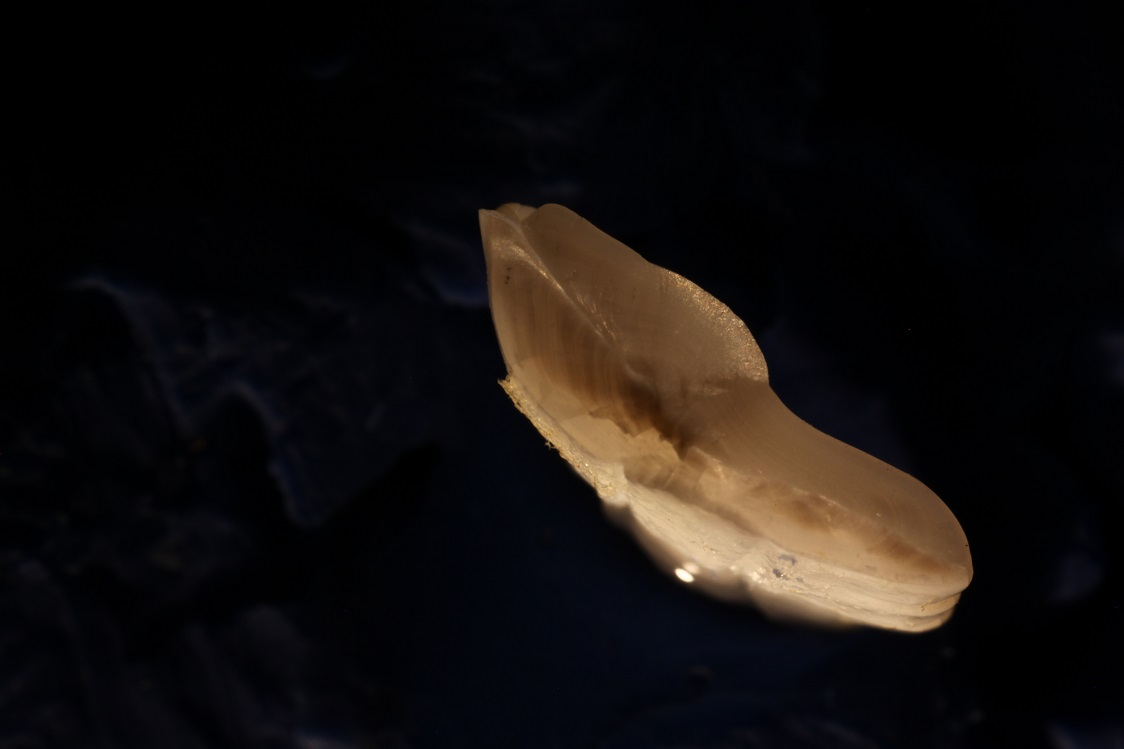
\includegraphics[width=0.45\textwidth]{outliers/IMG_0230_71.JPG}
  
  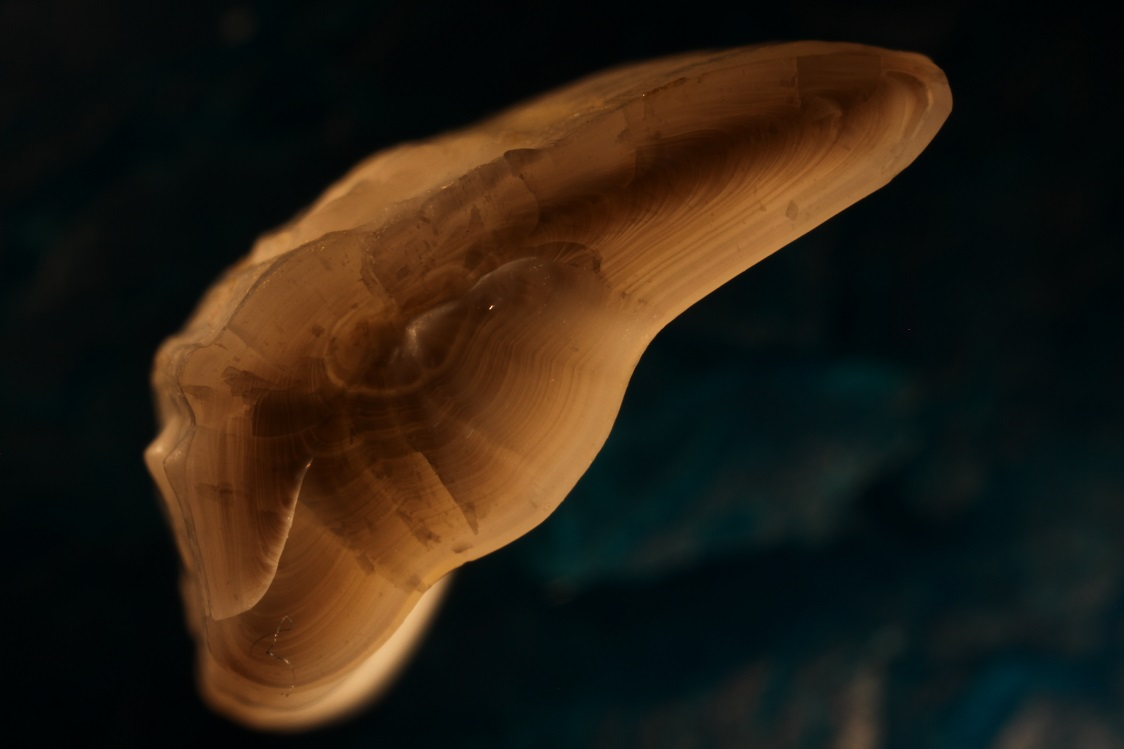
\includegraphics[width=0.45\textwidth]{outliers/IMG_0104_270.JPG} 
  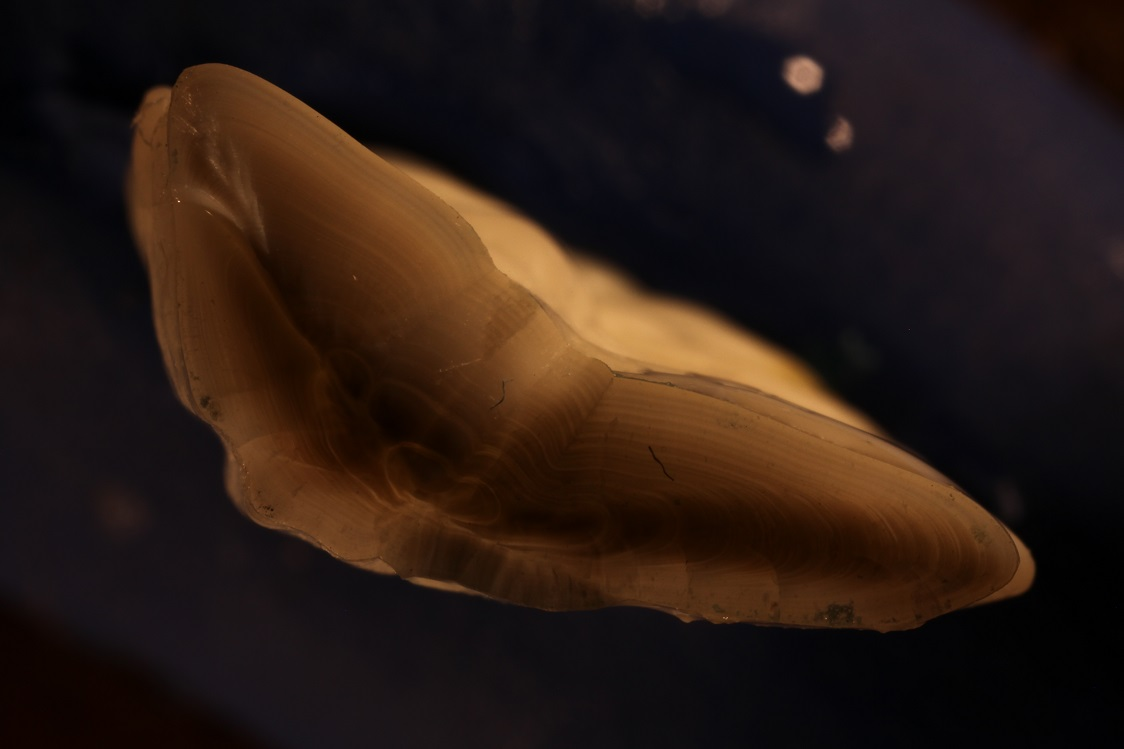
\includegraphics[width=0.45\textwidth]{outliers/IMG_0044_342.JPG}
  
  %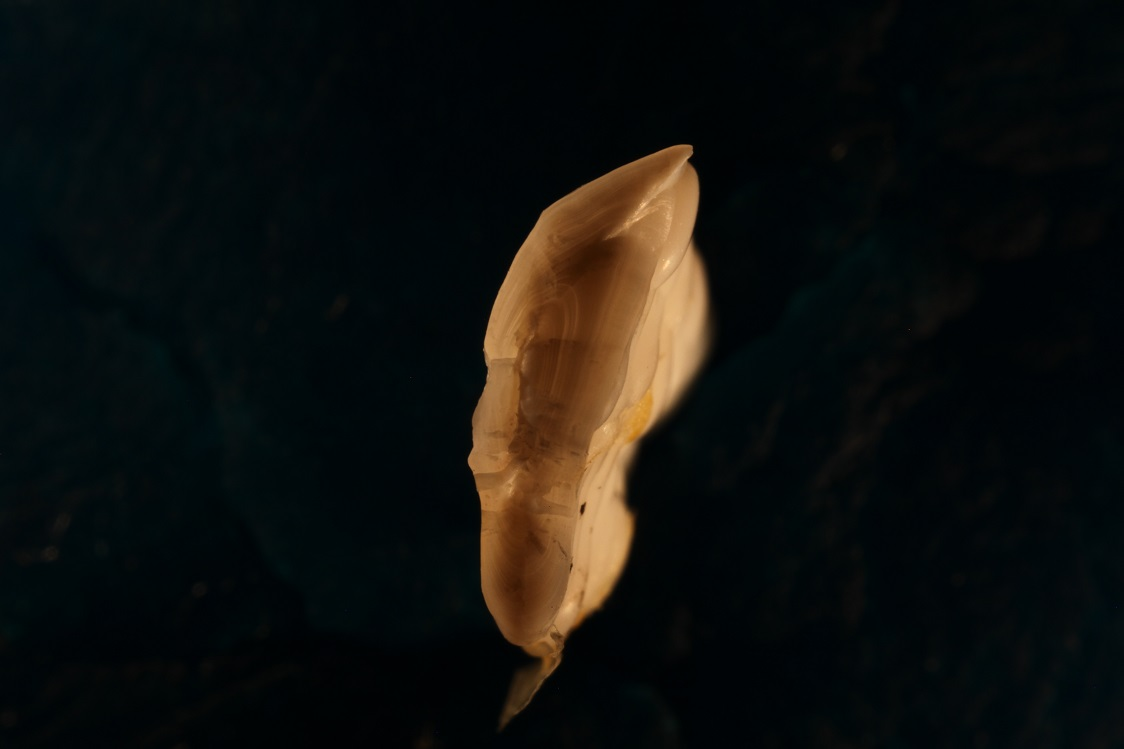
\includegraphics[width=0.45\textwidth]{outliers/IMG_0086_360.JPG}
  %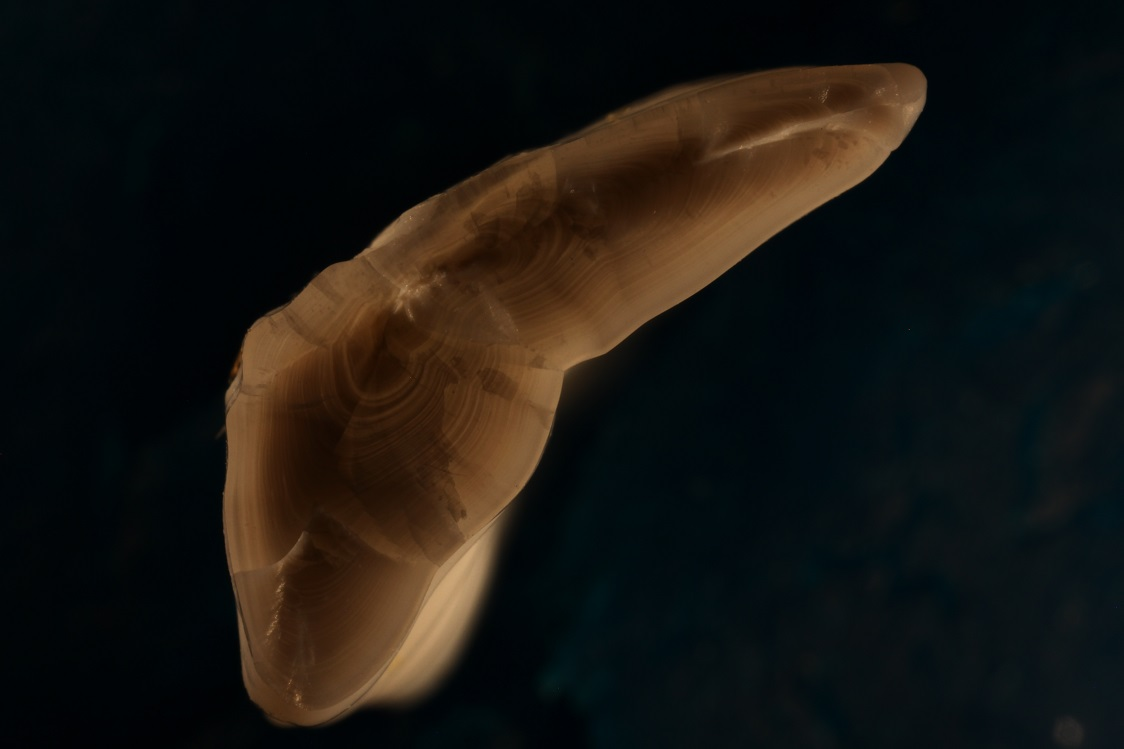
\includegraphics[width=0.45\textwidth]{outliers/IMG_0122_369.JPG}
  
    \caption{Example outlier images with index 13, 71, 279, 342
  %, 362 and 369
  from the test-set
  were mispredicted by between 25\% and 100\% of the models}
  \label{marker8}
\end{figure}

Some cod otoliths were outliers to all models and on all exposures (e.g. otoliths 71, 342, 362, and 369),
to a family of models and on all exposures (e.g. otoliths: 13, 423), 
to some models and on one exposure (E.g otolith 308), 
and to both families of models and on some exposures (\textit{E.g.} otolith 320).

We also observed that the number of  outliers did not correlate with model performance. \textit{E.g.}, B5-min, and B6-mid which had 7 and 9 outliers, but the best  accuracy. While B4-max with the lowest accuracy (70.9\%) had the least number of outliers with only 6 mispredictions.

\subsection{Correlation of predictions and cluster analysis}

The correlation of models on the test-set predictions given in Figure \ref{marker9} in supplementary information shows that the models strongly correlate in outlier predictions. 
The correlation from all the predictions on the test set varied between 0.988 to 0.999, with the lowest correlation found between B5-min and Medium-min. 

Hierarchical clustering (HCA) of the models found 3 clusters. One cluster contained B5-min and B6-middle, which werethe two best performing models. A second cluster contained of all the EfficientNetV2 models, and a third cluster contained the rest of the models (Figure \ref{marker10}, and \ref{marker9}).

The two least correlated models, B5-min and Medium-min, which had Pearson's correlation of 0.988 showed strongly correlated predictions also on a sub-year scale (Figure \ref{marker12}).  This means that the model output is not simply a Gaussian or other symmetric distribution around the correct (integral) value, but that the models identify characteristics of the input that lead them to classify it to a highly precise fractional value.

\begin{figure}[hbtp!]
  \centering
  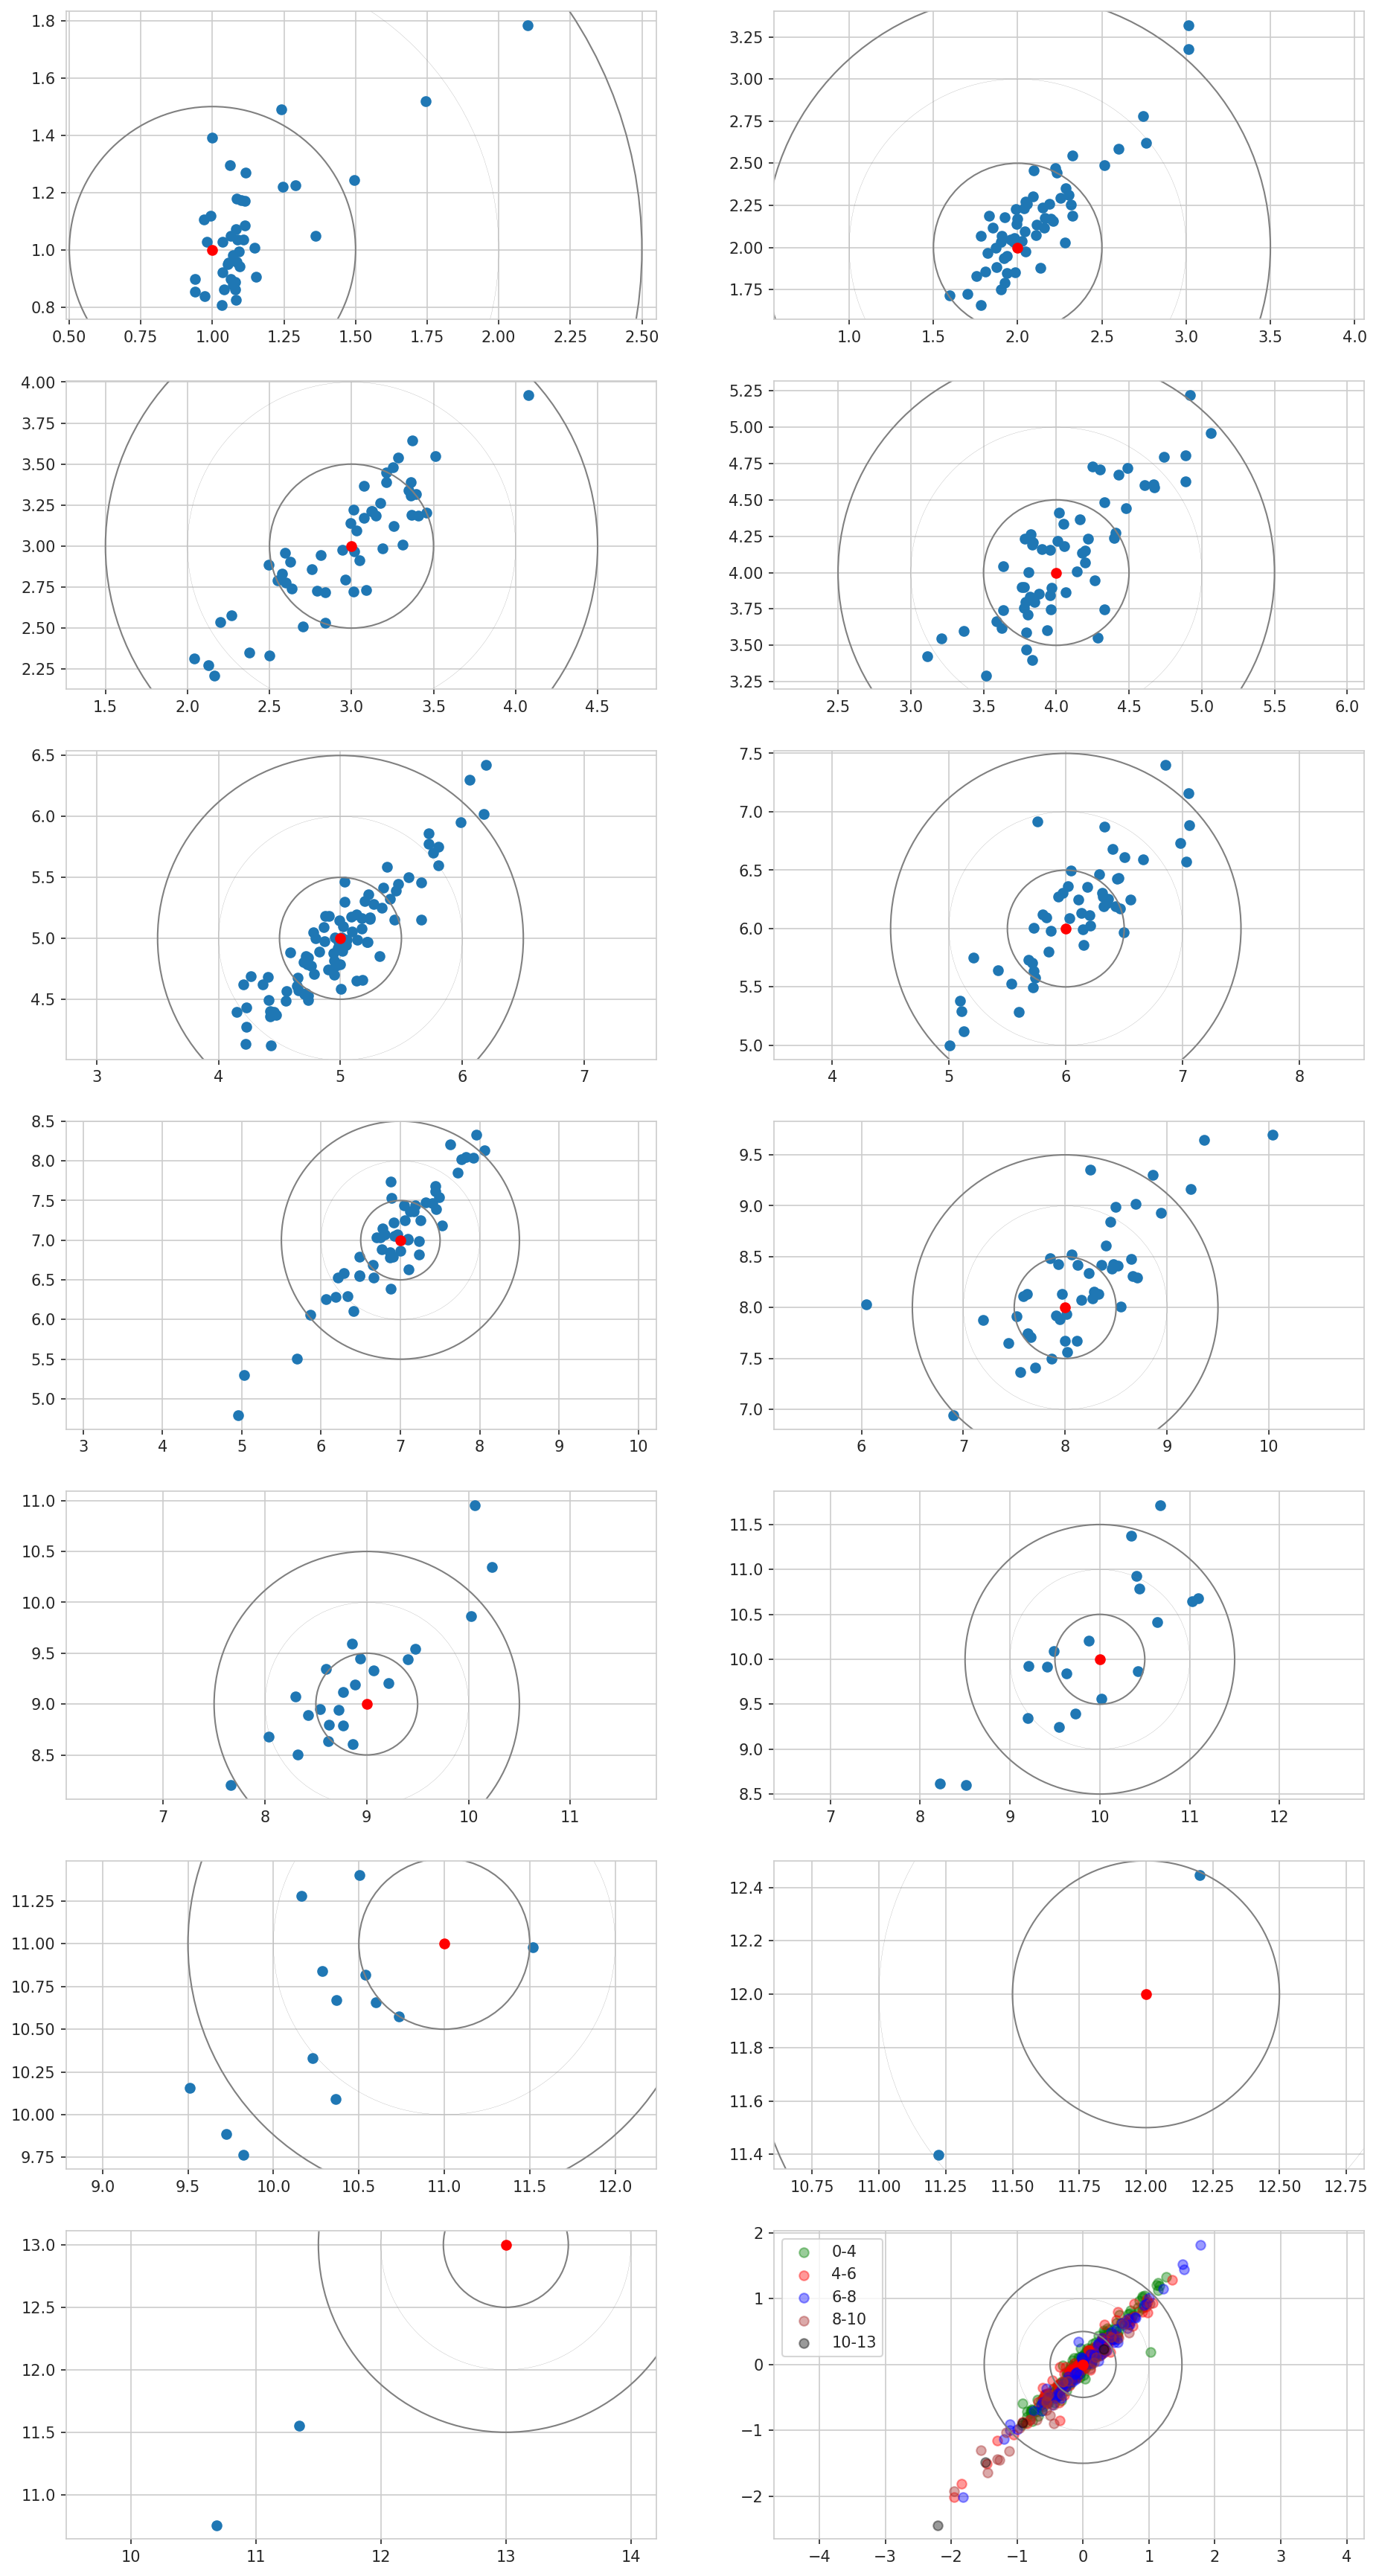
\includegraphics[scale=0.35]{results/eda/m_min_x_b5_min.png}
    \caption{Comparison of age estimates predicted by Medium-min (x axis, years) and B5-min (y axis, years) as age-specific scatter plots, and in aggregate for all age groups  in the bottom right panel.  The circles show age differences of 0.5 and 1.5 years.}
  \label{marker12}
\end{figure}

\subsection{Comparison of CNN with human readers}
Variations in percentage agreement between age classes showed similar patterns in both CNN-based predictions and human readers, with generally decreasing agreement with age (Figure \ref{marker19}). Within each age class, percentage agreement from CNN-based predictions was lower than the average for multiple human readers and increasingly so for the older age classes. However, they often remained within or close to the range of percentage agreement observed across all readers for all otoliths of a given age class. 

\begin{figure}[hbt!]
  \centering
  \includegraphics[scale=0.12]{results/CNNHuman_comparison_errorbars.jpg}
    \caption{Comparison of mean percentage agreement within each age class for two sets of otoliths: the CNN-predictions on the test set (black); an internal age reading of 100 cod otoliths involving 7 readers (gray). Numbers indicate the total number of readings for each age class (with 1 reading per otolith for the CNN but 7 readings for the workshop). Error bars indicate the range of percentage agreement between readers for all otoliths of a given age class.}
  \label{marker19}    
\end{figure}

\section{Discussion}
We successfully trained and tested machine learning methods on images of broken otoliths, and achieved a maximum accuracy of 78.6\% with an ensemble consisting of six models, noting that the accuracy is the agreement between the read ages and the model predictions. 

\subsection{Accuracy across different age groups}

The age of the younger individuals was predicted with greater accuracy than those of older individuals by our models. Thus, the CNN appears to be particularly competent at aging cod otoliths of younger age. This is also  typical for expert readers who generally show the greatest accuracy for the youngest age classes which have fewer and clearer rings \citep{campana2001accuracy}. However, the reasons both humans and CNNs find the age of younger individuals easier to predict may not be the same. Human expert readers use various visual cues, prior knowledge, and background information to determine fish age, such as comparing ring counts on multiple axes and having intrinsic knowledge of the periodicity of opaque and translucent zones for a given species. In younger fish, the increments are usually wider and more clearly separated as fish -and consequently otolith- growth rates are maximal prior to maturity. Fish of age 1 are small and have comparatively small otoliths with a straightforward ring pattern made of one single finished opaque and translucent zone, and expert readers are unlikely to disagree on its interpretation.  On the other hand, a CNN architecture as used here identifies hierarchical patterns on different scales of the image from which it derives a value in the range of those provided in the training set. This means that unless specifically forced to do so, the algorithm may seek and interpret visual clues other than the rings human readers are trained to use.  A possible explanation for the higher prediction accuracy of younger fish is that age is related to the area the otolith covers relative to the total image size. Because the same camera settings were used, all images had the same dimension and calibration. For a species with moderately large adults such as Atlantic cod \citep{froese2022fishbase}, the otoliths will grow in size significantly faster during the first years and then slow down with approaching sexual maturity. As fish get older different growth trajectories will then lead to greater overlap in otolith sizes across different ages. It is therefore possible that the CNNs are not counting growth zones as human expert readers would, but rather that they synthesize all available patterns in the image to find recurring characteristics to the ages provided in the training set. The size of the area that the otoliths cover against the more uniform black background might for example be a very simple feature picked up by the CNNs yet with high predictive power for the youngest fish. , while the higher inter-individual variability and greater size overlap at older ages would affect the predictive accuracy of CNNs

The hypothesis that CNNs exploit other information than the growth zones is consistent with the findings of an earlier study where network activations inside a CNN were explored for images of Greenland halibut otoliths \citep{ordonez2020explaining}. Visualisation techniques were used to reveal the relative importance of attributes such as shape, inner structure, and size of the otoliths using activation maps. Importantly, the authors found that the CNN utilized information in pixels corresponding to annual increments to only a small extent.  To explore this possibility, we attempted to train a network using otolith silhouettes only, but were unable to achieve good performance.

\subsection{Importance of training set size relative to model performance}

It is commonly recognized that the performance of deep learning systems often improves with more training data \citep{lecun2015deep}. A crucial issue in machine learning projects is then determining the amount of training data needed to achieve a specific performance goal. In this study we utilized a somewhat large data set of around 5000 images, although the images were divided among a large range of age classes. In comparison, it is not uncommon for deep learning systems for image classification such as ImageNet to be trained on thousands of images for each class \citep{Russakovsky2015}. In this study, the use of transfer learning \citep{NIPS2014_5347} and augmentation yielded a significant performance boost but it is still likely that the network would provide more robust predictions with a larger training set. From a preliminary initial training not reported as part of this study, we trained a B4 network on about 2000 images and obtained an accuracy of around 60\%. When another 3000 images were added to the data set accuracy reached about 70\%. This could suggest that increasing our sample size would have further increased accuracy.


\subsection{The effect of image size}
The high-resolution $3744×5616$ cod otolith images were scaled down to between $380×380$ and $528×528$ pixels to match the requirements of the different EfficientNet architectures. This reduction in resolution may have affected the readability of finer-scale visual features such as growth rings. The fixed camera setup resulted in the background constituting a non-negligible proportion of the images, especially for smaller otoliths. 
This is especially true due to the curved or oval shape of the otolith, as a compressed image will not only have less pixels to work with but will also have a comparatively more important fraction of black background, which is effectively useless for age interpretation. Otoliths of other fish species like red mullet which have a more circular shape may be less sensitive to this problem \citep{Politikos}.
 Improvements might therefore be made by instead first isolating the otoliths from their background and cropping the image accordingly, in order to have a machine learning network trained on using exclusively the information contained within the area of interest. This would also limit information loss from image compression.


\subsection{Outliers and transparency}
The different networks were generally able to predict the age of otoliths with less than a one-year deviation from the labelled values. It is noteworthy that predicted ages were similar across different models and errors of more than a year were only seen in 2\% of the predictions on the test set. Closer inspection revealed that such errors were often caused by otolith images with poor readability, in particular drastic changes in exposure or visual damages and interruptions on the reading axis. 

Interestingly, for one of these images, the predicted age was correct, and a reexamination by an expert revealed that the initial annotation was wrong by two years. While the previous results suggest that the network may not have relied entirely on ring patterns for estimating age, this correct prediction of a wrongly assigned age shows that it is still utilizing cues that are somewhat age-specific. Model behaviour was also similar across all networks on single predictions of outliers: four  were identified in all of the models, suggesting they must have learned the same features.

\subsection{Effects of image exposure on predictive power}

Among the 17 models trained and explored in this study, models trained on low-exposure images gave the best performance. Models trained on the medium-exposure images and the nine-channel images also performed better than the high-exposure images. The reason for this is not entirely clear. While low-exposure images may seem too dark and thereby hide useful visual details from a human point of view, our results show that it is not necessarily the case for an algorithm operating on finer-scale pixel values. It is likely that overexposure causes burnout and irreversible loss of information while underexposed images retain their information and only suffer from introduced noise.

\subsection{Effects of 9-channel composite images and architecture size}
Combining all 3 exposures into a 9-channel image did not perform better even if more information was available to these CNNs. The EfficientNetV2 models trained on these performed similarly to models trained on single-exposure images. 
The variance of predictions on 9-channel images was noticeably lower than for regular images, meaning the CNNs were more certain in their prediction even when the  prediction was wrong.

We also found that the newer and larger EfficientNetV2 architecture did not stand out as better than the EfficientNetV1 models. On the contrary, some of the best models were the smaller ones of B4, B5, and B6. This could be due to the size of our data set not being large enough to utilizing all the parameters in the larger models. Larger networks are generally able to better explore a larger data set, such as ImageNet, through training. 

\subsection{Utilising model ensembles.}
We observed slight improvements in performance when an ensemble of models was used for prediction. The use of numerous models in ensembles resulted in large numbers of combinations of model predictions with varying accuracy. Some combinations achieved higher accuracy than others (close to 79\% for some combinations of six and seven models). However, the mean ensemble prediction accuracy for a given number of models showed that five models or more in combination resulted in accuracy just above 75\%. Five models thus seem to be sufficient and there could be minimal gain in precision in combining larger numbers of models. Interestingly, ensembles combining models with higher variance resulted in better predictions. This can indicate that if models are too similar in individual predictions, the averaging effect ("wisdom of the crowds") will not play out in the same way as when models with higher variance are combined. Remarkably, many predictions only disagreed with a small decimal fraction. This could imply that the models learned the same features in the otolith images.

\subsection{Comparison of CNN with human readers}
The comparison of age-specific percentage agreement in CNN-based predictions with those from an internal age reading workshop showed that our models may achieve similar agreement with human readers. While the numerical results are not directly comparable in the sense that two different sets of otoliths were read, the trends in mean precision across age groups were similar. 
Of particular interest is the fact that the mean percentage agreement for our CNN-based predictions for a given age group generally fell within or close to the range of percentage agreement for all otoliths of a given age class seen between all readers involved in an age reading workshop. This may indicate that while machine-based methods have not yet have the predictive accuracy of an expert human reader, their estimates still fall within the expected range and may not be easily distinguishable from those of traditional readers. Further testing should be conducted to assess whether this is consistent, for example by conducting a multi-reader aging event that includes undisclosed machine-based estimates of the same samples and monitoring how they compare and whether they can be picked out by human readers. 


\subsection{Resource efficiency}
Even if networks are reliable and trustworthy a remaining question will still be whether there are significant cost benefits of deploying a ML framework for age reading of otoliths. Despite fast progress, the results remain mixed and often yield lower precision and consistency than those obtained by trained expert readers, which limits the application of automated methods in real conditions. However, one aspect that is often under-considered by such studies is the practical time and cost benefits that implementing a functional ML framework would provide. As noted by Fisher and Hunter (2018) \citen{Fisher} in their review of digital techniques for otolith analysis, “costs for human and machine ageing systems are broadly similar since a large part of the cost is associated with preparing the otolith sections”. As such, the net benefit of automated ageing routines is directly dependent on the ability to scale performance using a comparatively smaller number of samples than expert readers or, alternatively, to train them on “rougher” data that can be produced faster and at a more efficient cost. Our study brings a net improvement toward this resource-efficient inclusion of machine-driven analysis to age reading, as our networks were trained exclusively on imaged broken otoliths. Whereas sectioned material requires time and laboratory resources to embed, section, and prepare the samples for imaging, breaking otoliths can be done immediately following collection from the fish. This means that images and age estimates could potentially be produced directly at sea, or at least processed in bulk as soon as the vessel and data are brought back to land. 

Also, CNNs can be applied without high additional cost or even be incorporated into the routine protocols, but add a new value e.g., reading consistency check, time-drift evaluations, inter-reader comparisons (how much ‘off’ is each reader when compared to the CNN predictions, even if not compared with the same otolith samples), etc.  The advantages of ensemble predictions will also be easier to gain with networks. Ensembles of several expert readers are highly resource-demanding – especially when scaling to huge datasets – while an ensemble of, say eight versus three networks only requires a little bit more computation.

We see the process of CNN implementation as an evolution of the protocols, with an intensive phase of model development and training. Through gradual improvement of model reliability, CNNs could emerge as a complementary supportive tool for traditional age estimations. The integration of those technologies could help scale the capacity of age reading experts and improve the sampling of biological data and monitoring of various fish stocks.

While the exact features used by the networks may differ from those interpreted by human readers, one may be content with a trained network as a black box relying entirely on its empirical accuracy. Deep learning techniques are particularly powerful in detecting patterns in data \citep{lecun2015deep}, and whether the networks actually detect and count annual increments as the defining features or not, a causal relationship between what the network attends to and the structure of the otoliths is likely. If the network does not use growth zones as the primary features for prediction, this means that it found useful correlating patterns unavailable or not obvious to the human eye. This was demonstrated in the case of Greenland halibut otoliths where the shape of the otoliths seemed to be the defining characteristic correlated with age \citep{ordonez2020explaining}. Machine learning frameworks may therefore be used as complementary age readers to experts participating in otolith image interpretation workshops, as informative input playing part of additional background information, or relied upon as autonomous age readers without a subjective bias specific to increment identification and counting. As efforts to develop machine-assisted frameworks increase, an important question to ask is therefore whether they are to be trained at replicating human methodology for specific tasks or instead given the freedom to generate new and often not easily visualised methods. 

\subsection{Conclusion}
Our results demonstrate that the use of deep learning techniques in the analysis of otoliths have a major potential for facilitating automation.  Standard model architectures trained on sufficient training data specific to the use case can accurately predict age from images of broken otoliths. We believe that carefully trained CNNs could become a major component in automated pipelines that require minimal processing and could be able to produce near at sea age estimates.  In addition, algorithmic age estimates could serve as a useful reference for training and evaluating expert readers.

When developing the CNN framework for the automatic age estimation, we found that the B4 architectures were quick to train and that they performed well. Ensemble approaches can also be considered if the increased computing effort is not a constraint to the automation process, as they can provide  more robust and higher-performing predictions. For a quick-to-train ensemble, B5 and Medium might be added. Our results also indicate that the use of slightly under-exposed images may be beneficial.

\section{Acknowledgements}

We thank Jane Godiksen and age readers and technicians from the Demersal Fish research group for providing otolith age estimates and images used for this study. We thank Erlend Langhelle for providing insight into the image-taking-protocol and age interpretation of cod otoliths.

\bibliographystyle{apalike}
\bibliography{references}

\pagebreak

\section{Supplementary information}
\subsection{Hyper-parameters}
\addcontentsline{toc}{section}{Appendices}

\centering
\begin{table}[hbt!]
    \caption{Hyper-parameters on each model}
    \begin{tabular}{ |l|c|c|c|c|c| } \hline 
    Param/CNN & B4 & B5 & B6 & Medium & Large  \\ \hline
    \texttt{train\char`_batch\char`_size} & 8 & 8 & 16 & 8 & 8 \\ 
    \texttt{img\char`_size} & 380 & 456 & 528 & 384 & 384 \\
    \texttt{val\char`_img\char`_size} & 380 & 456 & 528 & 384 & 384 \\
    \texttt{steps\char`_per\char`_epoch} & 1600 & 1600 & 1600 & 1600 & 1600\\
    \texttt{epochs} & 150 & 150 & 250 & 450 & 450 \\
    \texttt{early\char`_stopping} & - & - & - & 40 & 40 \\
    \texttt{early\char`_stopping\char`_patience} &  14 & 14 & 22 & - & - \\
    \texttt{reduceLROnPlateau\char`_patience} & 7 & 7 & 11 & - &  - \\
    \hline
    \end{tabular}
    \label{table2}
    \footnotesize{\\ Medium all-, and min-exposures was run with \texttt{steps\char`_per\char`_epoch}=160 \\
    B6 has epochs=150, \texttt{early\char`_stopping\char`_patience}=14, and
    \texttt{reduceLROnPlateau\char`_patience}=7 \\
    B4 min was run with \texttt{img\char`_size}=456}\\
\end{table}

\begin{table}[hbt!]
\caption{Hyper-parameters on all models, TensorFlow only (B4,B5, B6), and PyTorch only (Medium and Large)}
\begin{tabular}{ |l|c|c|c| } \hline
\texttt{Parameter} & Value & TensorFlow & PyTorch  \\  \hline
\texttt{learning\char`_rate} & 1e-05 & v & v\\
\texttt{n\char`_fold} & 10 & v & v \\
\texttt{test\char`_size} & 0.1 & v & v \\
\texttt{in\char`_chans} & 3 or 9 & v & v  \\ \hline
\texttt{reduceLROnPlateau\char`_factor} & 0.2 & v & x\\
\texttt{which\char`_exposure} & min, medium, max & v & x  \\ \hline
\texttt{scheduler} & CosineAnnealingLR & x & v \\
\texttt{T\char`_max} & 10 & x & v \\
\texttt{min\char`_lr} & 1e-06 & x & v \\
\texttt{weight\char`_decay} & 1e-06 & x & v \\
\texttt{which\char`_exposure} & min, medium, max, all & x & v \\
\hline
\end{tabular}
\label{table3}
{\footnotesize
\texttt{in\char`_chans} is the number of channels as input for the model. It was either 3 for an RGB image or 9 channels for 3 images.}
\end{table}

\subsection{Model architecture}
 
\begin{figure}[ht!]
  \centering
    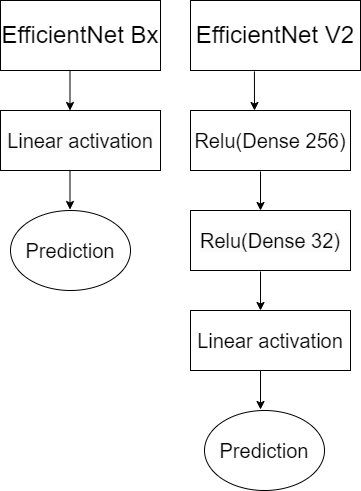
\includegraphics[width=0.80\textwidth]{results/eda/archtecture.png}
    \caption{Diagram showing the changes made to the two architecture families}
    \label{fig99}
\end{figure}

% END hyperparameters #######################

\pagebreak

\section{Descriptive Statistics}

\begin{figure}[ht!]
  \centering
    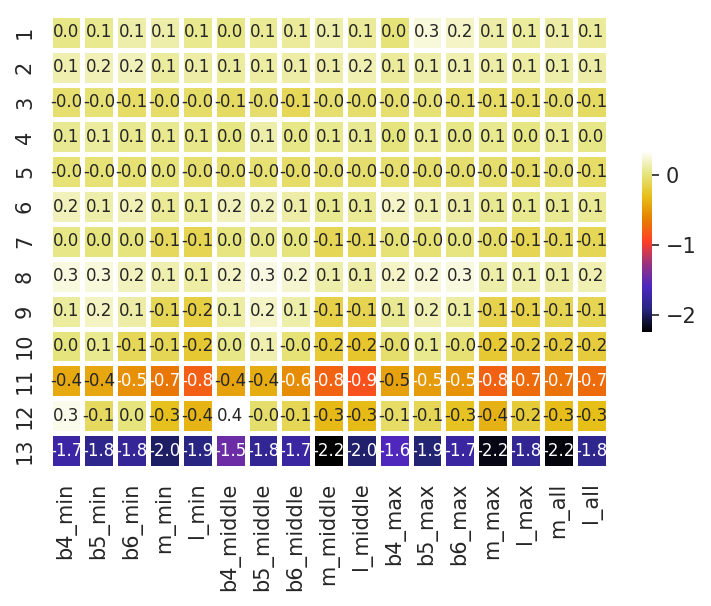
\includegraphics[width=0.80\textwidth]{results/eda/age_mean.png} %0.82\label{fig:7a}
    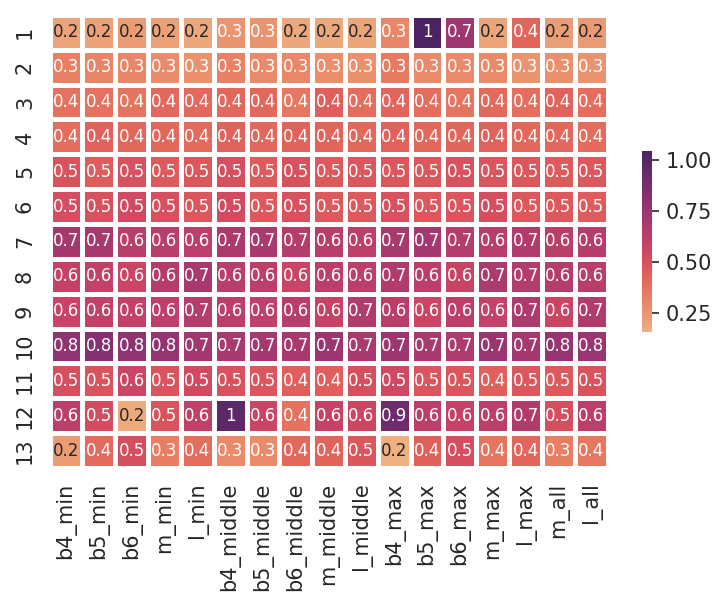
\includegraphics[width=0.80\textwidth]{results/eda/age_std.png}  %0.82
    \label{fig7b}
    \caption{Model mean (top) and standard deviation (bottom) of residual test set prediction by age class}
\end{figure}
% END Model mean and standard dev

\pagebreak

\subsection{Model accuracy and MSE per fold}

\centering
\begingroup
\captionsetup[table]{hypcap=false}
\captionof{table}{MSE per CNN per fold}
\rotatebox{90}{
    \begin{tabular}{|l|l|l|l|l|l|l|l|l|l|l|l|l|}
    \hline
        CNN/fold  & 1    & 2    & 3    & 4    & 5    & 6    & 7    & 8    & 9    & 10   & ens. & Mean \\ \hline
        B4,min    & .320 & .318 & .306 & .313 & .322 & .314 & .315 & .316 & .306 & .302 & .277 & .313 \\ \hline
        B4,middle & .344 & .328 & .316 & .334 & .326 & .320 & .355 & .326 & .313 & .325 & .285 & .329 \\ \hline
        B4,max    & .340 & .317 & .318 & .347 & .336 & .336 & .336 & .320 & .354 & .336 & .291 & .334 \\ \hline
        B5,min    & .324 & .322 & .325 & .336 & .291 & .314 & .320 & .331 & .33  & .317 & .277 & .321 \\ \hline
        B5,middle & .308 & .286 & .315 & .349 & .332 & .310 & .280 & .275 & .331 & .288 & .273 & .307 \\ \hline
        B5,max    & .472 & .302 & .437 & .459 & .432 & .366 & .356 & .441 & .438 & .418 & .359 & .412 \\ \hline
        B6,min    & .325 & .329 & .334 & .293 & .312 & .290 & .320 & .300 & .276 & .306 & .272 & .309 \\ \hline
        B6,middle & .323 & .301 & .312 & .268 & .294 & .266 & .309 & .311 & .278 & .289 & .262 & .295 \\ \hline
        B6,max    & .435 & .306 & .306 & .270 & .390 & .321 & .411 & .321 & .294 & .448 & .305 & .350 \\ \hline
        m,min     & .292 & .292 & .294 & .275 & .298 & .304 & .304 & .331 & .307 & .295 & .273 & .299 \\ \hline
        m,middle  & .287 & .302 & .307 & .332 & .288 & .276 & .277 & .294 & .304 & .278 & .278 & .295 \\ \hline
        m,max     & .337 & .297 & .302 & .291 & .315 & .347 & .338 & .321 & .313 & .283 & .289 & .314 \\ \hline
        m,all     & .289 & .299 & .303 & .284 & .292 & .287 & .303 & .288 & .289 & .294 & .273 & .293 \\ \hline
        l,min     & .267 & .316 & .269 & .270 & .322 & .332 & .280 & .307 & .303 & .299 & .280 & .297 \\ \hline
        l,middle  & .300 & .332 & .320 & .300 & .272 & .302 & .294 & .285 & .307 & .285 & .275 & .300 \\ \hline
        l,max     & .322 & .295 & .324 & .353 & .295 & .306 & .271 & .292 & .380 & .299 & .286 & .314 \\ \hline
        l,all     & .285 & .293 & .283 & .274 & .286 & .325 & .272 & .283 & .277 & .295 & .271 & .287 \\ \hline
        Mean      & .328 & .308	& .316 & .315 &	.318 & .313 & .314 & .314 & .318 & .315	& .284 & .316 \\ \hline
    \end{tabular}
    \label{table11}    
}
\endgroup

\pagebreak
\centering
\begingroup
\captionsetup[table]{hypcap=false}
\captionof{table}{Accuracy per CNN per fold}
\rotatebox{90}{
    \begin{tabular}{|l|l|l|l|l|l|l|l|l|l|l|l|l|}
    \hline
        CNN/fold   & 1    & 2    & 3    & 4    & 5    & 6    & 7    & 8    & 9    & 10   & ens. & Mean \\ \hline
        B4, min    & 69.9 & 68.9 & 68.7 & 68.3 & 68.9 & 70.1 & 69.7 & 66.8 & 68.9 & 72.4 & 72.8 & 69.3 \\ \hline
        B4, middle & 68.5 & 69.3 & 73.0 & 68.5 & 67.8 & 68.2 & 67.2 & 67.2 & 68.3 & 69.5 & 71.5 & 68.8 \\ \hline
        B4, max    & 64.1 & 68.2 & 67.2 & 66.2 & 67.8 & 69.5 & 67.2 & 69.3 & 66.2 & 65.2 & 70.9 & 67.1 \\ \hline
        B5, min    & 71.8 & 69.1 & 69.3 & 66.8 & 73.6 & 70.7 & 66.2 & 68.3 & 69.5 & 68.7 & 74.4 & 69.4 \\ \hline
        B5, middle & 70.3 & 72.0 & 67.8 & 66.6 & 67.4 & 69.9 & 71.8 & 71.5 & 68.2 & 72.2 & 73.4 & 69.8 \\ \hline
        B5, max    & 71.3 & 71.1 & 67.4 & 73.2 & 66.4 & 68.9 & 64.1 & 69.1 & 68.7 & 71.8 & 73.2 & 69.2 \\ \hline
        B6, min    & 68.3 & 68.5 & 66.4 & 72.4 & 70.7 & 70.9 & 69.3 & 69.3 & 72.0 & 68.9 & 73.4 & 69.7 \\ \hline
        B6, middle & 68.5 & 69.9 & 67.6 & 73.6 & 72.8 & 72.0 & 68.0 & 69.3 & 72.0 & 71.1 & 74.4 & 70.5 \\ \hline
        B6, max    & 70.5 & 68.2 & 65.2 & 73.2 & 69.1 & 67.8 & 68.0 & 68.0 & 72.8 & 68.5 & 71.5 & 69.1 \\ \hline
        m, min     & 71.1 & 71.1 & 69.5 & 73.4 & 71.8 & 70.9 & 70.9 & 69.7 & 70.1 & 71.5 & 74.0 & 71.0 \\ \hline
        m, middle  & 71.3 & 70.1 & 70.1 & 70.9 & 71.7 & 71.8 & 72.0 & 71.3 & 69.3 & 71.8 & 72.4 & 71.0 \\ \hline
        m, max     & 68.9 & 70.1 & 70.3 & 71.3 & 70.7 & 68.5 & 69.7 & 68.0 & 69.1 & 71.8 & 71.3 & 69.8 \\ \hline
        m, all     & 71.7 & 70.7 & 69.3 & 71.3 & 71.8 & 71.8 & 71.3 & 71.7 & 71.1 & 70.7 & 74.0 & 71.1 \\ \hline
        l, min     & 72.4 & 69.7 & 71.5 & 70.8 & 71.3 & 71.3 & 70.9 & 69.9 & 71.1 & 70.5 & 72.0 & 71.0 \\ \hline
        l, middle  & 68.7 & 68.0 & 69.7 & 71.8 & 71.1 & 71.1 & 69.7 & 70.5 & 71.1 & 72.0 & 72.8 & 70.4 \\ \hline
        l, max     & 71.1 & 70.1 & 69.9 & 74.2 & 72.8 & 71.1 & 72.2 & 71.1 & 71.1 & 70.1 & 72.4 & 71.4 \\ \hline
        l, all     & 71.8 & 71.7 & 71.8 & 71.7 & 71.7 & 68.0 & 73.2 & 71.7 & 73.0 & 71.5 & 72.2 & 71.6 \\ \hline
        Mean       & 70.0 & 69.8 & 69.1 & 70.8 & 70.4 & 70.1 & 69.5 & 69.6 & 70.1 & 70.5 & 72.7 & 70.0 \\ \hline
    \end{tabular}
\label{table12}    
}
\endgroup
% END Accuracy per CNN per fold

\pagebreak
\subsection{Predicted age class for all models and ground truth}
\centering
\begin{figure}[ht!]
  \centering
  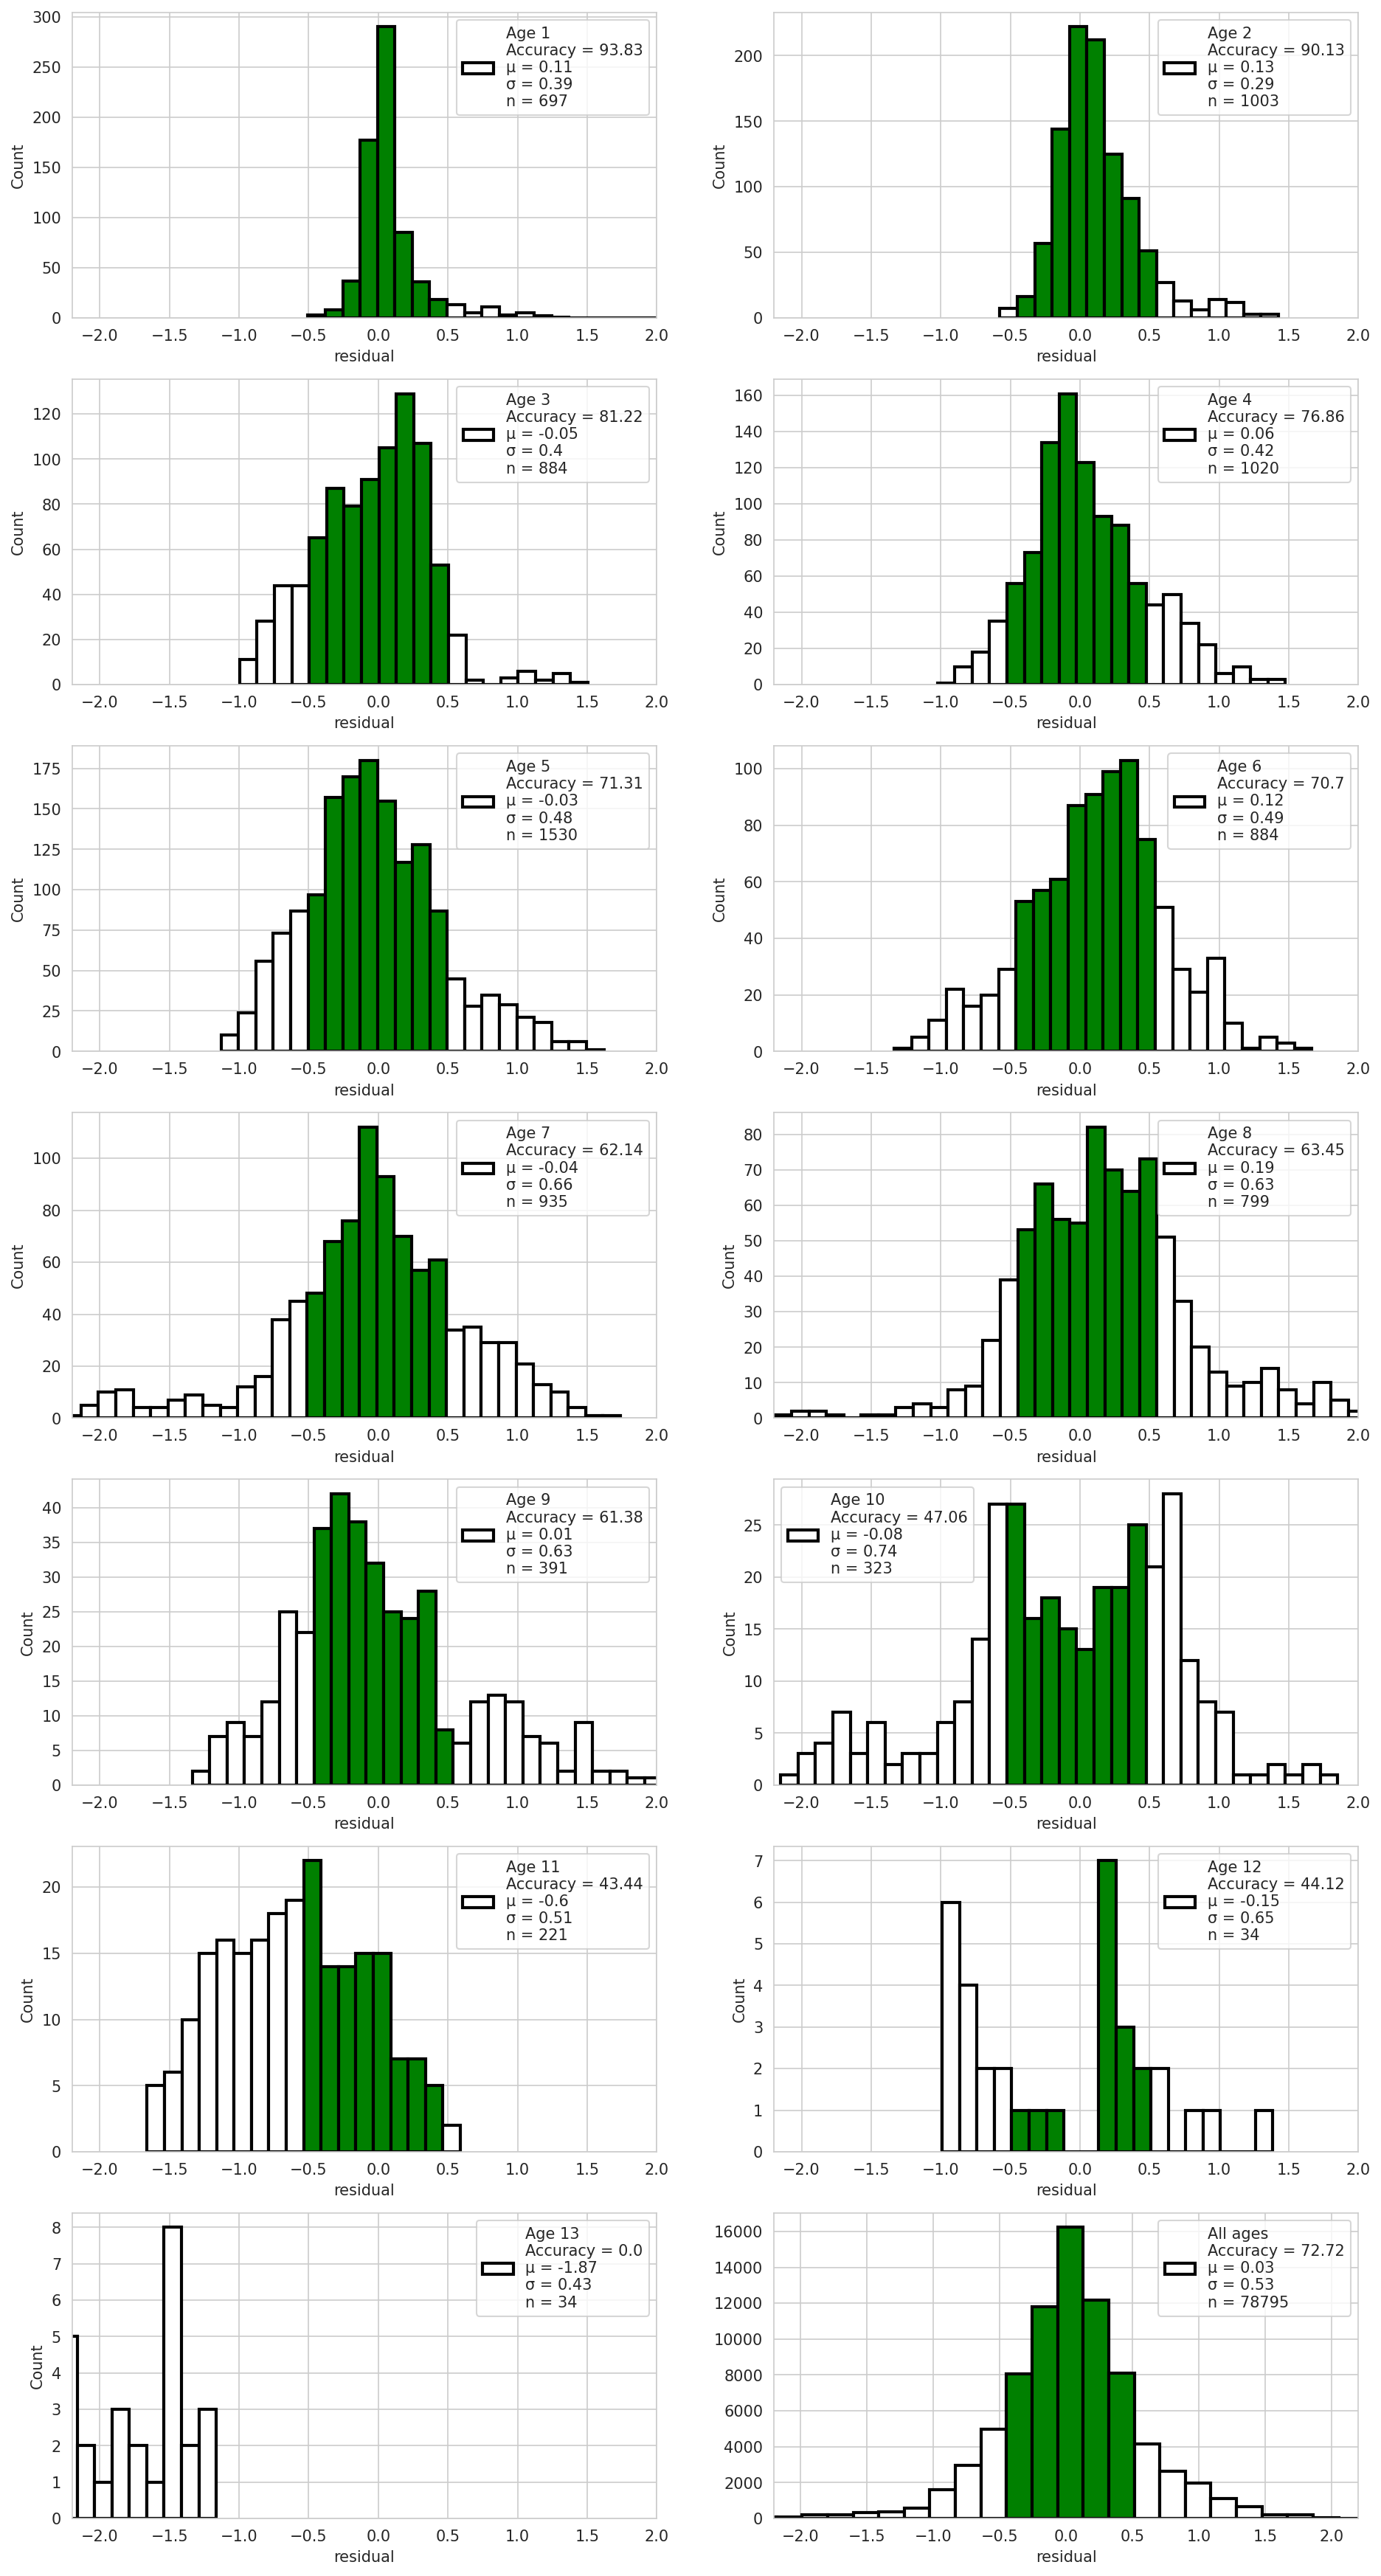
\includegraphics[scale=0.30]{results/eda/acc_by_age_dist_hist3.png}
    \caption{Predictions by age class from the average of all models. The green region shows the correctly classified age after rounding. The axis is fixed, hence outliers that differ from the true age by more than two years will not be visible.}
  \label{marker6}    
\end{figure}
% END predictited age class diagram

\pagebreak

\section{Outliers}


    \centering
    \begingroup
    \captionsetup[table]{hypcap=false}
    \captionof{table}{Predictions error with residual of more than 1.5 years per model per index in test-set}
    \rotatebox{90}{
    \setlength\tabcolsep{1.5pt} % default value: 6pt
    \renewcommand{\arraystretch}{0.8}
    \begin{tabular}{|l|l|l|l|l|l|l|l|l|l|l|l|l|l|l|l|l|l|l|l|l|l|l|l|l|}
    \hline
        Idx           & 13  & 17 & 47 & 48 & 71 & 92 & 154 & 270 & 279 & 308 & 312 & 320 & 334 & 342 & 362 & 369 & 393 & 418 & 423 &444 & 462 & 481 & 502 &  Count \\ \hline
        B4-min        & 9.8 &    &    & ~  &5.1 & ~  &     &11.7 & 9.9 & ~   & ~   & 5.5 &     &11.1 & 5.1 & 8.2 & ~   & ~   &  ~  &  ~  & ~  & ~   & ~   &  8  \\ \hline
        B4-mid        & 9.7 &    &    & ~  &5.4 & ~  &     &     &10.2 & ~   &~    & 5.4 & 7.5 &11.3 & 4.9 & 8.3 &10.6 & 9.5 &  ~  &  ~  & ~  & ~   & ~   &  10 \\ \hline
        B4-max        & 9.6 &    &    & ~  &5.0 & ~  &     &     &10.4 & ~   &~    &     &     &11.3 & 5.0 & 8.2 & ~   & ~   &  ~  &  ~  & ~  & ~   & ~   &  6  \\ \hline
        B5-min        & 9.6 &    &    & ~  &4.8 & ~  &     &11.7 & 9.7 & ~   &~    & ~   &     &10.8 & 5.3 & ~   & ~   & ~   &  ~  &11.0 & ~  & ~   & ~   &  7  \\ \hline
        B5-mid        & 9.8 &    &    & ~  &6.7 &11.5&     &11.8 & 9.8 & ~   &~    &     &     &10.9 & 5.3 & 8.4 & ~   & ~   &  ~  &10.7 & ~  & ~   & ~   &  9  \\ \hline
        B5-max        & 9.8 &    &    & ~  &4.5 &11.5&     &     & 9.6 & 7.7 &~    &     &     &10.6 & 5.1 & 8.3 & ~   & ~   &  ~  & ~   & ~  & ~   & ~   &  8* \\ \hline
        B6-min        & 9.7 &    &    &7.6 &5.1 & ~  &     & ~   & 9.7 & ~   &~    & ~   &     &10.7 & 5.2 & 7.9 &10.8 &10.7 &  ~  & ~   & ~  & ~   & 9.4 &  9  \\ \hline
        B6-mid        & 9.6 &    &    & ~  &5.1 & ~  &     &11.5 & 9.7 & ~   &~    & ~   &     &10.8 & 5.2 & 8.3 &10.8 & ~   &  ~  &     & ~  & ~   & 9.4 &  9  \\ \hline
        B6-max        & 9.8 &    &    & ~  &5.2 & ~  &     &     &     & 5.7 &~    &     &     &10.7 & 5.2 & 8.2 &10.6 & ~   &  ~  &     &6.5 & ~   & 9.4 &  9**  \\ \hline
        m-min         &     &    &    & ~  &5.0 &11.3&     &     &10.0 & ~   &~    &     &     &10.7 & 5.0 & 8.2 & ~   & ~   & 6.0 & ~   & ~  & ~   & ~   &  7  \\ \hline
        m-mid         & ~   &    &    & ~  &4.9 &11.2&     & ~   &10.0 & ~   &~    & ~   &     &10.3 & 5.1 & 8.2 & ~   &     &  ~  & ~   & ~  & ~   & ~   &  6 \\ \hline
        m-max         &     &    &6.5 & ~  &5.1 &11.2&8.7  &     &10.2 & ~   &~    &     &     &10.5 & 5.1 & 8.1 & ~   & ~   & 6.3 & ~   & ~  & ~   & ~   &  9  \\ \hline
        m-all         &     &    &    & ~  &5.0 &11.2&     &     &10.1 & ~   &~    &     &     &10.5 & 5.3 & 8.2 & ~   & ~   & 6.2 & ~   & ~  & 8.4 & ~   &  8  \\ \hline
        l-min         &     &    &    & ~  &5.1 &11.5&     &     & 9.8 & ~   &9.3  &     &     &10.7 & 5.2 & 8.3 & ~   & ~   & 5.1 & ~   & ~  & ~   & ~   &  8  \\ \hline
        l-mid         & ~   &    &    & ~  &5.0 & ~  &     & ~   & 9.8 & ~   &9.4  & 5.5 &     &10.6 & 5.2 & 8.1 &10.5 &     & 6.0 & ~   & ~  & ~   & ~   &  9  \\ \hline
        l-max         &     &9.5 &    & ~  &5.1 & ~  &     &     & 9.9 & 3.6 &~    & 5.4 &     &10.8 & 5.1 & 8.2 & ~   & ~   & 5.9 & ~   & ~  & 8.4 & ~   &  10  \\ \hline
        l-all         & ~   &9.3 &    & ~  &5.0 & ~  &     & ~   & 9.8 & ~   &     & ~   &     &10.8 & 5.2 & 8.0 &10.5 &     & 6.2 & ~   & ~  & 8.5 & ~   &  9  \\ \hline
        Age           & 8   &  8 & 8  & 6  & 7  & 13 & 7   & 10  & 8   & 1   &11   & 7   & 6   & 13  & 7   & 10  & 9   & 11  & 8  & 11   & 5   & 10 & 11  &  -  \\ \hline
        Count         & 9   &  2 & 1  & 1  &17  & 7  & 1   & 4   & 16  & 3   &2    & 2   & 1   &17   & 17  & 17  & 6   & 2   & 7  &  2   & 1   & 3  & 3   & 141 \\ \hline
        As pct        & 53  & 12 & 6  & 6  &100 & 41 & 6   & 24  & 94  & 18  &12   & 12  & 6   &100  & 100 & 100 & 35  & 12  & 41 &  12  & 6   & 18 & 18  & -  \\ \hline
    \end{tabular}
\label{table10}
}
\endgroup

\pagebreak
% Comments on outliers
    \centering
    \begingroup
    \captionsetup[table]{hypcap=false}
    \captionof{table}{Comments on the most frequently mispredicted otolith images}
    \setlength\tabcolsep{1.5pt} % default value: 6pt
    \renewcommand{\arraystretch}{0.8}
    \begin{tabular}{|l|p{13cm}|}
    \hline
        Idx & Comment \\ \hline
        13  & Labeled 8 years, and read as 10 years by the B-models (EfficentNet).
              The quality of the exposures was good, but there was a lot of split rings in the middle. \\ \hline
        71  & Labeled 7 years, and read as 5 years by all models. 
              The exposures were very bright on all three axes, and the dorsal axis had a break line (fissure or physical break), and the plane was out of focus. \\ \hline
        279 & Labeled as 8 years, and read as 10 years by almost all models except B6-max. 
              The exposures were of good quality, but there were split rings in the middle. \\ \hline
        308 & Labeled as 1 year, and read as 8 years, 6 years and 4 years by B5-max, b6-max, and Large-max respectively.  
              The exposures were of good quality and the predicted age is obviously wrong. \\ \hline
        342 & Labeled as 13 years, and read as 11 years by all models. The quality of the exposures was good. 
              The inner section is dark on the ventral side, the distal side is light, and the dorsal side has a break line.  \\ \hline
        362 & Labeled as 7 years, and read as 5 years by all models. This image is mislabeled. The otolith is obviously 5 years old.\\ \hline
        369 & Labeled as 10 years, and read as 8 years by all models except B5-min.   
              The quality of the exposures was good, but it had split rings in the middle on bright exposures, and the contrast is strong. \\ \hline
        393 & Labeled as 9 years, and was read as 11 years by B4-middle, all B6 exposures and Large-middle and -all. 
              The middle and min exposures were too dark. Max exposure was nice. \\ \hline
        423 & Labeled as 8 years, and read as 6 years by all the EfficentNetV2 models except Medium-middle. 
              The quality of the images was bad. All the exposures were over-exposed. \\ \hline  
    \end{tabular}
\label{table10b}
\endgroup

\pagebreak





\pagebreak

\section{Ensembles by simple average}
\centering

Table \ref{table6} shows the number of combinations of models that exist
of tuples, triplets, and so on labeled with the heading "Coeff", then
the best ensemble-average accuracy on the given number of combinations,
and then the model numbers that produced the best combinations. Model number can be
translated to model name using Table \ref{table1}. Table \ref{table7}
shows the same information but selected to minimize MSE. 

\begin{table}[hbt!]
\caption{The table shows the model family as columns and image exposure as rows. The numbering of models is used in reference to ensembles.}
\begin{tabular}{ |l|c|c|c|c|c|c| }
\hline
CNN family / & \multicolumn{3}{c|}{EfficientNet} & \multicolumn{2}{c|}{EfficientNetV2} \\
Image exposure & B4 & B5 & B6 &Medium &Large  \\ 
\hline
Minimum & 1 & 2 & 3 & 4 & 5  \\ 
Medium & 6 & 7 & 8 & 9 & 10  \\ 
Maximum & 11 & 12 & 13 & 14 & 15  \\ 
9 channels & - & - & - & 16 & 17  \\ 
\hline
\end{tabular}
\label{table1}
\end{table}

\begin{center}
\begin{table}[hbt!]
\caption{Binomial combinations of simple average of ensembles accuracy}
\begin{tabular}{ |l|l|l|l|l| }
\hline
Coeff & \#Comb & Best & Mean & Ensemble (see table \ref{table1}) \\ \hline
2 & 136 &    75.9 & 74.1 & (2, 5) \\ \hline
3 & 680 &    77.5 & 74.6 & (1, 3, 4) \\ \hline
4 & 2380 &   77.9 & 74.9 & (1, 2, 3, 4) \\ \hline
5 & 6188 &   77.9 & 75.1 & (1, 2, 3, 4, 11) \\ \hline
6 & 12376 &  78.6 & 75.2 & (1, 2, 3, 4, 8, 11) \\ \hline
7 & 19448 &  78.1 & 75.2 & (1, 2, 3, 4, 7, 8, 11) \\ \hline
8 & 24310 &  77.5 & 75.2 & (1, 2, 3, 4, 7, 8, 10, 11) \\ \hline
9 & 24310 &  77.5 & 75.3 & (1, 2, 3, 6, 7, 8, 9, 11, 17) \\ \hline
10 & 19448 & 77.1 & 75.2 & (1, 2, 3, 6, 7, 8, 9, 10, 12, 13) \\ \hline
11 & 12376 & 76.9 & 75.2 & (1, 2, 3, 4, 6, 7, 8, 10, 11, 13, 16) \\ \hline
12 & 6188 &  76.7 & 75.2 & (1, 3, 4, 7, 8, 10, 11, 13, 14, 15, 16, 17) \\ \hline
13 & 2380 &  76.3 & 75.1 & (1, 3, 4, 7, 8, 9, 10, 11, 13, 14, 15, 16, 17) \\ \hline
14 & 680 &   75.9 & 75.1 & (1, 2, 3, 4, 5, 8, 9, 10, 11, 12, 13, 14, 16, 17) \\ \hline
15 & 136 &   75.7 & 75.0 & (1, 2, 3, 4, 5, 7, 8, 9, 10, 12, 13, 14, 15, 16, 17) \\ \hline
16 & 17 &    75.5 & 75.0 & (1, 2, 3, 4, 5, 6, 7, 8, 9, 10, 12, 13, 14, 15, 16, 17) \\ \hline
17 & 1 &     74.8 & 74.8 & (1, 2, 3, 4, 5, 6, 7, 8, 9, 10, 11, 12, 13, 14, 15, 16, 17) \\ \hline
\end{tabular}
\label{table6}
\end{table}
\end{center}

\begin{center}
\begin{table}[hbt!]
\caption{Binomial combinations of simple average of ensembles MSE}
\begin{tabular}{ |l|l|l|l|l| }
\hline
Coeff & \#comb & best & Mean & Ensemble  (see table \ref{table1}) \\ \hline
2 & 136 &    0.250 & 0.265 & (3, 17) \\ \hline
3 & 680 &    0.246 & 0.259 & (1, 3, 5) \\ \hline
4 & 2380 &   0.245 & 0.256 & (1, 3, 5, 7) \\ \hline
5 & 6188 &   0.245 & 0.254 & (1, 3, 4, 7, 17) \\ \hline
6 & 12376 &  0.244 & 0.252 & (1, 2, 3, 5, 8, 16) \\ \hline
7 & 19448 &  0.244 & 0.251 & (1, 2, 3, 4, 5, 8, 11) \\ \hline
8 & 24310 &  0.244 & 0.251 & (1, 2, 3, 4, 5, 8, 11, 17) \\ \hline
9 & 24310 &  0.244 & 0.250 & (1, 2, 3, 4, 5, 7, 8, 11, 17) \\ \hline
10 & 19448 & 0.244 & 0.250 & (1, 2, 3, 4, 5, 7, 8, 11, 16, 17) \\ \hline
11 & 12376 & 0.245 & 0.250 & (1, 2, 3, 4, 5, 7, 8, 10, 11, 13, 16) \\ \hline
12 & 6188 &  0.245 & 0.249 & (1, 2, 3, 4, 5, 6, 7, 8, 10, 11, 16, 17) \\ \hline
13 & 2380 &  0.245 & 0.249 & (1, 2, 3, 4, 5, 6, 7, 8, 10, 11, 13, 16, 17) \\ \hline
14 & 680 &   0.245 & 0.249 & (1, 2, 3, 4, 5, 6, 7, 8, 9, 10, 11, 13, 16, 17) \\ \hline
15 & 136 &   0.246 & 0.249 & (1, 2, 3, 4, 5, 6, 7, 8, 9, 10, 11, 13, 15, 16, 17) \\ \hline
16 & 17 &    0.247 & 0.248 & (1, 2, 3, 4, 5, 6, 7, 8, 9, 10, 11, 13, 14, 15, 16, 17) \\ \hline
17 & 1 &     0.248 & 0.248 & (1, 2, 3, 4, 5, 6, 7, 8, 9, 10, 11, 12, 13, 14, 15, 16, 17) \\ \hline
\end{tabular}
\label{table7}
\end{table}
\end{center}
%\pagebreak

\centering
\begin{center}
\begin{table}[hbt!]
\caption{Comparison of the mean of all the 17 models (mean) with a total accuracy of 72.7\% and 
the best ensemble model (Best Ens.) with a total accuracy of 78.6\%. In all age groups, the
ensemble improves on the mean-model accuracy except 13 year-olds.}
\setlength\tabcolsep{3.5pt} % default value: 6pt
\begin{tabular}{ |l|c|c|c|c|c|c|c|c|c|c|c|c|c|c| }
\hline
Age        & 1    & 2    & 3    & 4    & 5    & 6    & 7    &  8   & 9  & 10   & 11   & 12   & 13   \\ \hline
Mean       & 93.8 & 90.1 & 81.2 & 76.9 & 71.3 & 70.7 & 62.1 & 63.5 & 61.4 & 47.1 & 43.4 & 44.1 & 0 \\ 
Best Ens.  & 95.1 & 93.2 & 84.6 & 80.0 & 78.9 & 78.9 & 65.6 & 76.6 & 69.6 & 52.6 & 61.5 & 50.0 & 0 \\ \hline
\end{tabular}
\label{table9}
\end{table}
\end{center}

\pagebreak

\subsection{Pearson correlation of each model on test-set predictions}
\centering

\begin{figure}[ht!]

  \centering
  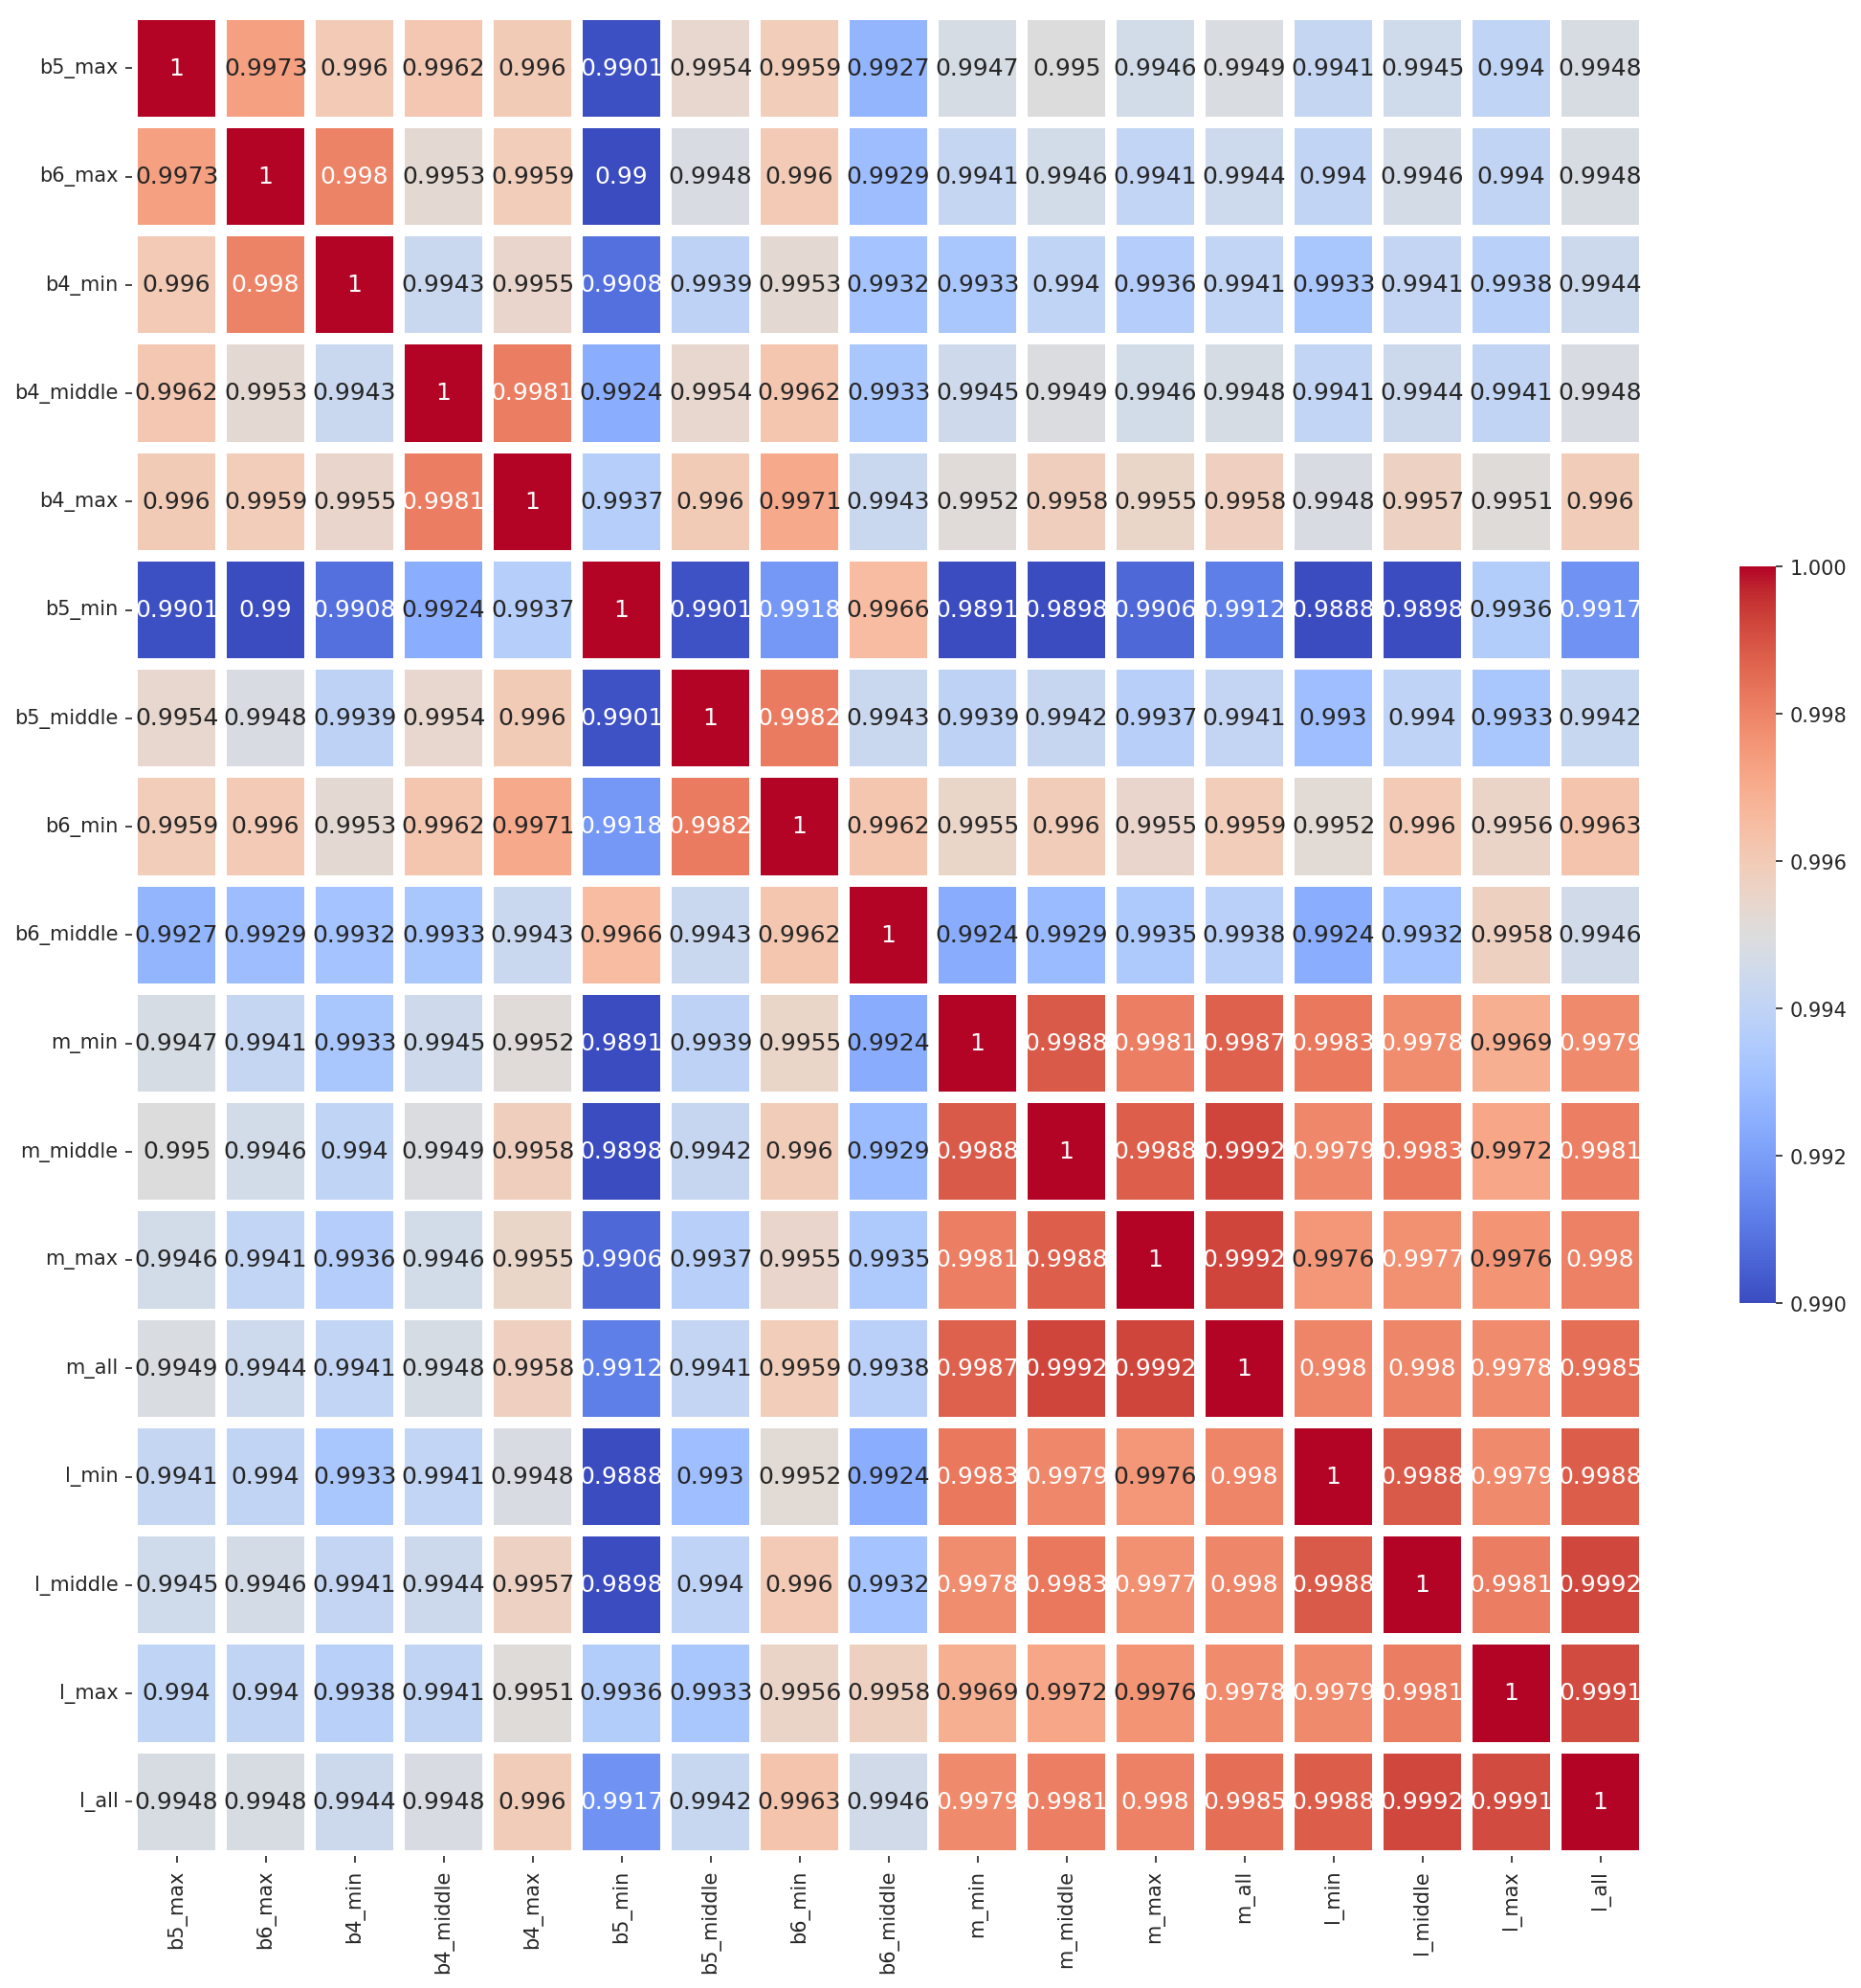
\includegraphics[scale=0.40]{results/eda/pearson_corr_models2.png}
    \caption{Pearson correlation of each model prediction on the test-set. The colors indicate the correlation coefficient, ranging from 0.99 (blue) to 1.00 (red).}
  \label{marker9}    
\end{figure}

\pagebreak

\subsection{T-statistics of each model vs model comparison on test-set prediction}
\centering
\begin{table}[hbt!]
\caption{T-statistics of each model vs other models (order as in table 1)}
    \setlength\tabcolsep{0.5pt} % default value: 6pt
    \renewcommand{\arraystretch}{0.8}
    \rotatebox{90}{
\begin{tabular}{ |l|c|c|c|c|c|c|c|c|c|c|c|c|c|c|c|c|c| }\hline
no & 2 & 3 & 4 & 5 & 6 & 7 & 8 & 9 & 10 & 11 & 12 & 13 & 14 & 15 & 16 & 17 \\ \hline 
1  & 0.873  & 0.588  & 0.00901 & 0.0074 & 0.465  & 0.56  & 0.158  & 0.00554 & 0.0967 & 0.00645  & 0.938  & 0.864  & 0.361   & 0.00385 & 0.00322 & 0.00199 \\
2  & -      & 0.768  & 0.0651 & 0.0679  & 0.462  & 0.723 & 0.284  & 0.0541  & 0.261  & 0.0173   & 0.851  & 0.782  & 0.601   & 0.0314  & 0.0407  & 0.0188 \\
3  & -      & -      & 0.0748 & 0.0755  & 0.251  & 0.931 & 0.381  & 0.0584  & 0.355  & 0.00417  & 0.649  & 0.566  & 0.826   & 0.0333  & 0.0408  & 0.0186 \\
4  & -      & -      & -      & 0.86   & 0.00312 & 0.132 & 0.517  & 0.933  & 0.273   & 2.04E-05 & 0.0823 & 0.0467 & 0.0433  & 0.516   & 0.756   & 0.306 \\
5  & -      & -      & -      & -      & 0.00293 & 0.139 & 0.562  & 0.764  & 0.282   & 2.65E-05 & 0.0875 & 0.0491 & 0.0348  & 0.381   & 0.546   & 0.205 \\
6  & -      & -      & -      & -      & -      & 0.256  & 0.0597 & 0.00219 & 0.0293 & 0.0414  & 0.668   & 0.698  & 0.118   & 0.00138 & 0.00147 & 0.000743 \\
7  & -      & -      & -      & -      & -      & -      & 0.46   & 0.111  & 0.46   & 0.00652  & 0.616   & 0.539  & 0.922   & 0.0646  & 0.084   & 0.0389 \\
8  & -      & -      & -      & -      & -      & -      & -      & 0.471  & 0.885  & 0.00104  & 0.26    & 0.199  & 0.422   & 0.289   & 0.388   & 0.189 \\
9  & -      & -      & -      & -      & -      & -      & -      & -      & 0.213  & 1.78E-05 & 0.0725  & 0.0396 & 0.0259  & 0.532   & 0.8     & 0.306 \\
10 & -      & -      & -      & -      & -      & -      & -      & -      & -      & 0.000173 & 0.25    & 0.177  & 0.371   & 0.115   & 0.139   & 0.0611 \\
11 & -      & -      & -      & -      & -      & -      & -      & -      & -      & -        & 0.057   & 0.0453 & 0.000753 & 9.82E-06 & 1.58E-05 & 5.84E-06 \\
12 & -      & -      & -      & -      & -      & -      & -      & -      & -      & -        & -       & 0.947  & 0.514   & 0.0447  & 0.0586  & 0.0294 \\
13 & -      & -      & -      & -      & -      & -      & -      & -      & -      & -        & -       & -      & 0.418   & 0.0234  & 0.0307  & 0.0145 \\
14 & -      & -      & -      & -      & -      & -      & -      & -      & -      & -        & -       & -      & -       & 0.0174  & 0.0134  & 0.00865 \\
15 & -      & -      & -      & -      & -      & -      & -      & -      & -      & -        & -       & -      & -       & -       & 0.643   & 0.711 \\
16 & -      & -      & -      & -      & -      & -      & -      & -      & -      & -        & -       & -      & -       & -       & -       & 0.375 \\

\end{tabular}
}
\label{table5c}
\end{table}

\end{document}
